% !TeX root = tcolorbox.tex
% include file of tcolorbox.tex (manual of the LaTeX package tcolorbox)
\clearpage
\section{程序库 \mylib{skins}}\label{sec:skins}%
\tcbset{external/prefix=external/skins_}%
加载本程序库的方式是使用宏包选项，或在导言区中使用：
\begin{dispListing}
\tcbuselibrary{skins}
\end{dispListing}
同时还会加载 \refPkg[tikzfill]{tikzfill.image} 宏包。

下文将介绍本程序库的通用设置与选项。
皮肤的完整目录见 \zvref{sec:skincatalog}。

\subsection{样式选项键}\label{subsec:addstyleoptions}
以下样式选项适用于所有使用 |path|、|pathfirst|、|pathmiddle|
或 |pathlast| 类型引擎的皮肤。
其中皮肤 \refSkin{enhanced} 支持\emph{全部}选项，
而 \refSkin{standard} 则\emph{一个也不支持}。

\begin{docTcbKey}{frame style}{=\meta{\texttt{\upshape tikz} keys}}{样式，无默认值}
  \meta{\texttt{\upshape tikz} 键}将被用于 \tikzname\ 路径命令中，
  以绘制文本框的\emph{边框}。\\
  当 \refKey{/tcb/frame engine} 设为
  |path|、|pathfirst|、|pathmiddle| 或 |pathlast| 时，本选项可用。
  对于 |standard|，本选项\emph{不可用}。
\begin{exdispExample*}{frame_style}{sbs,lefthand ratio=0.66}
\tcbset{colback=red!5!white,fonttitle=\bfseries}

\begin{tcolorbox}[enhanced,title=My title,
  frame style={left color=red!75!black,
               right color=blue!75!black}]
This is a \textbf{tcolorbox}.
\tcblower
This is the lower part.
\end{tcolorbox}
\end{exdispExample*}
\end{docTcbKey}


\begin{docTcbKey}{frame style image}{=\meta{file name}}{无默认值，初始未设置}
  用 \meta{文件名} 指定的外部图像填充边框。
\begin{exdispExample*}{frame_style_image}{sbs,lefthand ratio=0.66}
\tcbset{colback=red!5!white,fonttitle=\bfseries}

\begin{tcolorbox}[enhanced,title=My title,
  frame style image=blueshade.png]
This is a \textbf{tcolorbox}.
\tcblower
This is the lower part.
\end{tcolorbox}
\end{exdispExample*}
\end{docTcbKey}

\clearpage
\begin{docTcbKey}{frame style tile}{=\marg{graphics options}\marg{file name}}{无默认值，初始未设置}
  用 \meta{文件名} 指定的外部图像生成平铺图案来填充边框。
  \meta{图像选项}会传递给底层的 \docAuxCommand*{includegraphics} 命令。
\begin{exdispExample*}{frame_style_tile}{sbs,lefthand ratio=0.66}
\tcbset{colback=red!5!white,coltitle=red!30!black,
  opacityback=0.75,fonttitle=\bfseries}

\begin{tcolorbox}[enhanced,title=My title,
  frame style tile={width=1cm}{pink_marble.png}]
This is a \textbf{tcolorbox}.
\tcblower
This is the lower part.
\end{tcolorbox}
\end{exdispExample*}
\end{docTcbKey}


\begin{docTcbKey}{frame hidden}{}{样式，无取值}
  这是 |frame style={draw=none,fill=none}| 的快捷方式。
  根据所用皮肤的不同，本选项会关闭边框的绘制。
  也可改用 \refKey{/tcb/frame empty}。
\begin{exdispExample*}{frame_hidden}{sbs,lefthand ratio=0.66}
\tcbset{colback=red!5!white,colframe=red!75!black,
  fonttitle=\bfseries,coltitle=black}

\begin{tcolorbox}[enhanced,title=My title,
  frame hidden]
This is a \textbf{tcolorbox}.
\tcblower
This is the lower part.
\end{tcolorbox}
\end{exdispExample*}
\end{docTcbKey}


\begin{docTcbKey}{interior style}{=\meta{\texttt{\upshape tikz} keys}}{样式，无默认值}
  \meta{\texttt{\upshape tikz} 键}将被用于 \tikzname\ 路径命令中，
  以绘制文本框的\emph{内部}。该内部同时用于带标题和不带标题的版本。\\
  当 \refKey{/tcb/interior titled engine}
  或 \refKey{/tcb/interior engine} 设为
  |path|、|pathfirst|、|pathmiddle| 或 |pathlast| 时，本选项可用。
  对于 |standard|，本选项\emph{不可用}。
\begin{exdispExample*}{interior_style}{sbs,lefthand ratio=0.66}
\tcbset{colframe=red!75!black,fonttitle=\bfseries}

\begin{tcolorbox}[enhanced,title=My title,
  interior style={left color=red!20!white,
                  right color=yellow!50!white}]
This is a \textbf{tcolorbox}.
\tcblower
This is the lower part.
\end{tcolorbox}
\end{exdispExample*}
\end{docTcbKey}

\clearpage
\begin{docTcbKey}{interior style image}{=\meta{file name}}{无默认值，初始未设置}
  用 \meta{文件名} 指定的外部图像填充内部。
\begin{exdispExample*}{interior_style_image}{sbs,lefthand ratio=0.66}
\tcbset{colframe=red!75!black,fonttitle=\bfseries}

\begin{tcolorbox}[enhanced,title=My title,
  interior style image=goldshade.png]
This is a \textbf{tcolorbox}.
\tcblower
This is the lower part.
\end{tcolorbox}
\end{exdispExample*}
\end{docTcbKey}


\begin{docTcbKey}{interior style tile}{=\marg{graphics options}\marg{file name}}{无默认值，初始未设置}
  用 \meta{文件名} 指定的外部图像生成平铺图案来填充内部。
  \meta{图像选项}会传递给底层的 \docAuxCommand*{includegraphics} 命令。
\begin{exdispExample*}{interior_style_tile}{sbs,lefthand ratio=0.66}
\tcbset{colframe=red!75!black,fonttitle=\bfseries}

\begin{tcolorbox}[enhanced,title=My title,
  interior style tile={width=2cm}{crinklepaper.png}]
This is a \textbf{tcolorbox}.
\tcblower
This is the lower part.
\end{tcolorbox}
\end{exdispExample*}
\end{docTcbKey}


\begin{docTcbKey}{interior hidden}{}{样式，无取值}
  这是 |interior style={draw=none,fill=none}| 的快捷方式。
  根据所用皮肤的不同，本选项会关闭内部的绘制。
  也可改用 \refKey{/tcb/interior empty} 和/或 \refKey{/tcb/interior titled empty}。
\begin{exdispExample*}{interior_hidden}{sbs,lefthand ratio=0.66}
\tcbset{frame style={top color=red!20!white,
  bottom color=red!20!white!75!black},
  fonttitle=\bfseries,coltitle=black}

\begin{tcolorbox}[enhanced,title=My title,
  interior hidden]
This is a \textbf{tcolorbox}.
\tcblower
This is the lower part.
\end{tcolorbox}
\end{exdispExample*}
\end{docTcbKey}

\clearpage
\begin{docTcbKey}{segmentation style}{=\meta{\texttt{\upshape tikz} keys}}{样式，无默认值}
  \meta{\texttt{\upshape tikz} 键}将被用于 \tikzname\ 路径命令中，
  以绘制文本框的\emph{分隔线}。\\
  当 \refKey{/tcb/segmentation engine} 设为 |path| 时，本选项可用。
  对于 |standard|，本选项\emph{不可用}。
\begin{exdispExample*}{segmentation_style}{sbs,lefthand ratio=0.66}
\tcbset{colback=red!5!white,colframe=red!75!black,
  fonttitle=\bfseries}

\begin{tcolorbox}[enhanced,title=My title,
  segmentation style={double=white,draw=blue,
                  double distance=1pt,solid}]
This is a \textbf{tcolorbox}.
\tcblower
This is the lower part.
\end{tcolorbox}
\end{exdispExample*}
\end{docTcbKey}


\begin{docTcbKey}{segmentation hidden}{}{样式，无取值}
  这是 |segmentation style={draw=none,fill=none}| 的快捷方式。
  根据所用皮肤的不同，本选项会关闭分隔线的绘制。
  另见 \refKey{/tcb/lower separated}，它对大多数皮肤具有相同效果。
  也可改用 \refKey{/tcb/segmentation empty}。
\begin{exdispExample*}{segmentation_hidden}{sbs,lefthand ratio=0.66}
\tcbset{colback=red!5!white,colframe=red!75!black,
  fonttitle=\bfseries}

\begin{tcolorbox}[title=My title,
  enhanced,segmentation hidden]
This is a \textbf{tcolorbox}.
\tcblower
This is the lower part.
\end{tcolorbox}
\end{exdispExample*}
\end{docTcbKey}


\begin{docTcbKey}{title style}{=\meta{\texttt{\upshape tikz} keys}}{样式，无默认值}
  \meta{\texttt{\upshape tikz} 键}将被用于 \tikzname\ 路径命令中，
  以绘制文本框的\emph{标题区域}。\\
  当 \refKey{/tcb/title engine} 设为
  |path|、|pathfirst|、|pathmiddle| 或 |pathlast| 时，本选项可用。
  对于 |standard|，本选项\emph{不可用}。
\begin{exdispExample*}{title_style}{sbs,lefthand ratio=0.66}
\tcbset{colback=red!5!white,colframe=red!75!black,
  coltitle=blue!50!black,fonttitle=\bfseries}

\begin{tcolorbox}[enhanced,title=My title,
  title style={left color=blue!15!yellow,
               right color=red!85!black}]
This is a \textbf{tcolorbox}.
\tcblower
This is the lower part.
\end{tcolorbox}
\end{exdispExample*}
\end{docTcbKey}

\clearpage
\begin{docTcbKey}{title style image}{=\meta{file name}}{无默认值，初始未设置}
  用 \meta{文件名} 指定的外部图像填充标题区域。
\begin{exdispExample*}{title_style_image}{sbs,lefthand ratio=0.66}
\tcbset{colback=blue!5!white,colframe=blue!75!black,
  fonttitle=\bfseries}

\begin{tcolorbox}[enhanced,title=My title,
  title style image=blueshade.png]
This is a \textbf{tcolorbox}.
\tcblower
This is the lower part.
\end{tcolorbox}
\end{exdispExample*}
\end{docTcbKey}


\begin{docTcbKey}{title style tile}{=\marg{graphics options}\marg{file name}}{无默认值，初始未设置}
  用 \meta{文件名} 指定的外部图像生成平铺图案来填充标题区域。
  \meta{图像选项}会传递给底层的 \docAuxCommand*{includegraphics} 命令。
\begin{exdispExample*}{title_style_tile}{sbs,lefthand ratio=0.66}
\tcbset{colback=red!5!white,colframe=red!75!black,
  coltitle=blue!50!black,fonttitle=\bfseries}

\begin{tcolorbox}[enhanced,title=My title,
  title style tile={width=1cm}{pink_marble.png}]
This is a \textbf{tcolorbox}.
\tcblower
This is the lower part.
\end{tcolorbox}
\end{exdispExample*}
\end{docTcbKey}


\begin{docTcbKey}{title hidden}{}{样式，无取值}
  这是 |title style={draw=none,fill=none}| 的快捷方式。
  根据所用皮肤的不同，本选项会关闭标题背景的绘制。
  另见 \refKey{/tcb/title filled}，它具有类似效果。
  也可改用 \refKey{/tcb/title empty}。
\begin{exdispExample*}{title_hidden}{sbs,lefthand ratio=0.66}
\tcbset{colback=red!5!white,colframe=red!75!black,
  fonttitle=\bfseries}

\begin{tcolorbox}[title=My title,
  enhanced,title hidden]
This is a \textbf{tcolorbox}.
\tcblower
This is the lower part.
\end{tcolorbox}
\end{exdispExample*}
\end{docTcbKey}


\clearpage


\begin{docTcbKey}[][doc new=2015-01-14]{titlerule style}{=\meta{\texttt{\upshape tikz} keys}}{样式，无默认值}
  \meta{\texttt{\upshape tikz} 键}用于绘制标题线，
  即可选标题下方的一条线。线宽由 \refKey{/tcb/titlerule} 控制。
  也可直接将其设为较小的线宽，以与标准线组合产生混合效果。
  本选项以 \refKey{/tcb/underlay} 的形式实现。因此它不适用于
  \refSkin{standard} 和 \refSkin{standard jigsaw}，但适用于
  其他所有皮肤，例如 \refSkin{enhanced}。
  作为底层装饰，本选项可多次使用，并可由 \refKey{/tcb/no underlay} 移除。
\begin{exdispExample*}{titlerule_style_1}{sbs,lefthand ratio=0.66}
\begin{tcolorbox}[enhanced,
  colback=red!5!white,colframe=red!75!black,
  colbacktitle=red!50!yellow,fonttitle=\bfseries,
  title=My title,
  titlerule=1mm,
  titlerule style=yellow  ]
This is a \textbf{tcolorbox}.
\end{tcolorbox}
\end{exdispExample*}

\begin{exdispExample*}{titlerule_style_2}{sbs,lefthand ratio=0.66}
\begin{tcolorbox}[enhanced,
  colback=red!5!white,colframe=red!75!black,
  colbacktitle=red!50!yellow,fonttitle=\bfseries,
  title=My title,
  titlerule=1mm,
  titlerule style={yellow,line width=0.5mm}  ]
This is a \textbf{tcolorbox}.
\end{tcolorbox}
\end{exdispExample*}

\begin{exdispExample*}{titlerule_style_3}{sbs,lefthand ratio=0.66}
\begin{tcolorbox}[enhanced,
  colback=red!10!white,colframe=red!75!black,
  colbacktitle=red!50!yellow,fonttitle=\bfseries,
  frame hidden,
  title=My title,
  boxrule=0pt,titlerule=1mm,
  titlerule style=red!50!black  ]
This is a \textbf{tcolorbox}.
\end{tcolorbox}
\end{exdispExample*}

\begin{exdispExample*}{titlerule_style_4}{sbs,lefthand ratio=0.66}
%\usetikzlibrary{arrows.meta}
\begin{tcolorbox}[empty,
  coltitle=red!75!black,fonttitle=\bfseries,
  borderline horizontal={0.5mm}{0pt}{red!50!white},
  title=My title,
  titlerule style={red,
    arrows = {Hooks[arc=270]-Hooks[arc=270]}} ]
This is a \textbf{tcolorbox}.
\end{tcolorbox}
\end{exdispExample*}
\end{docTcbKey}

\clearpage

应用于边框、内部和标题背景的组合 \tikzname\ 样式，可供作者在自定义代码中使用。

\begin{docTikzKey}{tcb fill frame}{}{样式，无取值}
这是一个 \tikzname\ 样式，最终应用于文本框的\emph{边框}。

\begin{exdispExample*}{tcb_fill_frame}{sbs,lefthand ratio=0.66}
% \tcbuselibrary{hooks}
\tcbset{enhanced,colback=red!5!white,
  colframe=red!75!black,fonttitle=\bfseries,
  frame code app={\path[tcb fill frame]
    ([yshift=-2mm]frame.north)
        circle (8mm); }  }

\begin{tcolorbox}[title=My title]
This is a \textbf{tcolorbox}.
\tcblower
This is the lower part.
\end{tcolorbox}
\end{exdispExample*}
\end{docTikzKey}


\begin{docTikzKey}{tcb fill interior}{}{样式，无取值}
这是一个 \tikzname\ 样式，最终应用于文本框的\emph{内部}。

\begin{exdispExample*}{tcb_fill_interior}{sbs,lefthand ratio=0.66}
% \tcbuselibrary{hooks}
\tcbset{enhanced,colback=red!5!white,
  colframe=red!75!black,fonttitle=\bfseries,
  interior titled code app={\path[tcb fill interior]
      ([yshift=-0.1pt]interior.north east)
    --([yshift=3pt]interior.north)
    --([yshift=-0.1pt]interior.north west)
    --cycle;}  }

\begin{tcolorbox}[title=My title]
This is a \textbf{tcolorbox}.
\tcblower
This is the lower part.
\end{tcolorbox}
\end{exdispExample*}
\end{docTikzKey}


\begin{docTikzKey}{tcb fill title}{}{样式，无取值}
这是一个 \tikzname\ 样式，最终应用于文本框的\emph{标题区域}。

\begin{exdispExample*}{tcb_fill_title}{sbs,lefthand ratio=0.66}
% \tcbuselibrary{hooks}
\tcbset{enhanced,colback=red!5!white,
  colframe=red!75!black,fonttitle=\bfseries,
  colbacktitle=blue!75!black,
  title code app={\path[tcb fill title]
    (title) circle (5mm); }  }

\begin{tcolorbox}[title=My title]
This is a \textbf{tcolorbox}.
\tcblower
This is the lower part.
\end{tcolorbox}
\end{exdispExample*}
\end{docTikzKey}

\clearpage

\begin{docTikzKey}[][doc new=2025-07-07]{tcb fill lower bicolor}{}{样式，无取值}
这是一个 \tikzname\ 样式，当使用 \refSkin{bicolor} 皮肤时，
最终应用于文本框的\emph{下部内部}。

\begin{exdispExample*}{tcb_fill_lower_bicolor}{sbs,lefthand ratio=0.66}
% \tcbuselibrary{hooks}
% \usetikzlibrary{decorations.pathmorphing}
\tcbset{bicolor,colback=red!5!white,
  colbacklower=blue!15!white,
  colframe=red!75!black,fonttitle=\bfseries,
  segmentation code app={
    \path[tcb fill lower bicolor,
          decoration={zigzag,amplitude=1mm}]
      decorate {
          ([yshift=-0.1pt]segmentation.east)
        --([yshift=-0.1pt]segmentation.west) }
      --cycle;}  }

\begin{tcolorbox}[title=My title]
This is a \textbf{tcolorbox}.
\tcblower
This is the lower part.
\end{tcolorbox}
\end{exdispExample*}
\end{docTikzKey}



\clearpage
\subsection{带框标题选项键}\label{subsec:skinboxedtitle}

\subsubsection{带框标题的位置}
以下选项将标题文字放入一个独立的 \refCom{tcbox} 中。
此带框标题可通过 \refKey{/tcb/boxed title style} 独立于主文本框进行定制。
具体位置可由 \meta{带框标题选项} 调整。

\begin{docTcbKey}{attach boxed title to top left}{\colOpt{=\marg{boxtitle options}}}{样式，默认为空}
标题被放入一个 \refCom{tcbox} 中，并附着到主文本框的左上角。
\begin{exdispExample*}{attach_boxed_title_to_top_left}{sbs,lefthand ratio=0.66}
\begin{tcolorbox}[enhanced,title=My title,
  attach boxed title to top left]
  This is a \textbf{tcolorbox}.
\end{tcolorbox}
\end{exdispExample*}
\end{docTcbKey}

\begin{docTcbKey}[][doc new=2021-07-30]{attach boxed title to top text left}{\colOpt{=\marg{boxtitle options}}}{样式，默认为空}
标题被放入一个 \refCom{tcbox} 中，并附着到主文本框的左上角，
同时平移以使标题文字与框内文字对齐。
\begin{exdispExample*}{attach_boxed_title_to_top_text_left}{sbs,lefthand ratio=0.66}
\begin{tcolorbox}[enhanced,title=My title,
  attach boxed title to top text left]
  This is a \textbf{tcolorbox}.
\end{tcolorbox}
\end{exdispExample*}
\end{docTcbKey}

\begin{docTcbKey}{attach boxed title to top center}{\colOpt{=\marg{boxtitle options}}}{样式，默认为空}
标题被放入一个 \refCom{tcbox} 中，并附着到主文本框的顶部。
\begin{exdispExample*}{attach_boxed_title_to_top_center}{sbs,lefthand ratio=0.66}
\begin{tcolorbox}[enhanced,title=My title,
  attach boxed title to top center]
  This is a \textbf{tcolorbox}.
\end{tcolorbox}
\end{exdispExample*}
\end{docTcbKey}

\begin{docTcbKey}[][doc new=2021-07-30]{attach boxed title to top text right}{\colOpt{=\marg{boxtitle options}}}{样式，默认为空}
标题被放入一个 \refCom{tcbox} 中，并附着到主文本框的右上角，
同时平移以使标题文字与框内文字对齐。
\begin{exdispExample*}{attach_boxed_title_to_top_text_right}{sbs,lefthand ratio=0.66}
\begin{tcolorbox}[enhanced,title=My title,
  halign=right,
  attach boxed title to top text right]
  This is a \textbf{tcolorbox}.
\end{tcolorbox}
\end{exdispExample*}
\end{docTcbKey}


\begin{docTcbKey}{attach boxed title to top right}{\colOpt{=\marg{boxtitle options}}}{样式，默认为空}
标题被放入一个 \refCom{tcbox} 中，并附着到主文本框的右上角。
\begin{exdispExample*}{attach_boxed_title_to_top_right}{sbs,lefthand ratio=0.66}
\begin{tcolorbox}[enhanced,title=My title,
  attach boxed title to top right]
  This is a \textbf{tcolorbox}.
\end{tcolorbox}
\end{exdispExample*}
\end{docTcbKey}

\clearpage

\begin{docTcbKey}{attach boxed title to bottom left}{\colOpt{=\marg{boxtitle options}}}{样式，默认为空}
标题被放入一个 \refCom{tcbox} 中，并附着到主文本框的左下角。
\begin{exdispExample*}{attach_boxed_title_to_bottom_left}{sbs,lefthand ratio=0.66}
\begin{tcolorbox}[enhanced,title=My title,
  attach boxed title to bottom left]
  This is a \textbf{tcolorbox}.
\end{tcolorbox}
\end{exdispExample*}
\end{docTcbKey}


\begin{docTcbKey}[][doc new=2021-07-30]{attach boxed title to bottom text left}{\colOpt{=\marg{boxtitle options}}}{样式，默认为空}
标题被放入一个 \refCom{tcbox} 中，并附着到主文本框的左下角，
同时平移以使标题文字与框内文字对齐。
注意：即使存在\emph{下部}，此处对齐的仍是\emph{上部}。
\begin{exdispExample*}{attach_boxed_title_to_bottom_text_left}{sbs,lefthand ratio=0.66}
\begin{tcolorbox}[enhanced,title=My title,
  attach boxed title to bottom text left]
  This is a \textbf{tcolorbox}.
\end{tcolorbox}
\end{exdispExample*}
\end{docTcbKey}


\begin{docTcbKey}{attach boxed title to bottom center}{\colOpt{=\marg{boxtitle options}}}{样式，默认为空}
标题被放入一个 \refCom{tcbox} 中，并附着到主文本框的底部。
\begin{exdispExample*}{attach_boxed_title_to_bottom_center}{sbs,lefthand ratio=0.66}
\begin{tcolorbox}[enhanced,title=My title,
  attach boxed title to bottom center]
  This is a \textbf{tcolorbox}.
\end{tcolorbox}
\end{exdispExample*}
\end{docTcbKey}


\begin{docTcbKey}[][doc new=2021-07-30]{attach boxed title to bottom text right}{\colOpt{=\marg{boxtitle options}}}{样式，默认为空}
标题被放入一个 \refCom{tcbox} 中，并附着到主文本框的右下角，
同时平移以使标题文字与框内文字对齐。
注意：即使存在\emph{下部}，此处对齐的仍是\emph{上部}。
\begin{exdispExample*}{attach_boxed_title_to_bottom_text_right}{sbs,lefthand ratio=0.66}
\begin{tcolorbox}[enhanced,title=My title,
  halign=right,
  attach boxed title to bottom text right]
  This is a \textbf{tcolorbox}.
\end{tcolorbox}
\end{exdispExample*}
\end{docTcbKey}


\begin{docTcbKey}{attach boxed title to bottom right}{\colOpt{=\marg{boxtitle options}}}{样式，默认为空}
标题被放入一个 \refCom{tcbox} 中，并附着到主文本框的右下角。
\begin{exdispExample*}{attach_boxed_title_to_bottom_right}{sbs,lefthand ratio=0.66}
\begin{tcolorbox}[enhanced,title=My title,
  attach boxed title to bottom right]
  This is a \textbf{tcolorbox}.
\end{tcolorbox}
\end{exdispExample*}
\end{docTcbKey}


\clearpage
\begin{docTcbKey}[][doc new=2016-02-26]{attach boxed title to top}{\colOpt{=\marg{boxtitle options}}}{样式，默认为空}
  这是一个便捷样式，用于模拟标准标题。
  它使用 \refKey{/tcb/attach boxed title to top center}
  和 \refKey{/tcb/minipage boxed title}，并调整带框标题的尺寸以匹配基础文本框。
\begin{dispExample*}{sbs,lefthand ratio=0.66}
\begin{tcolorbox}[enhanced,title=My title,
  attach boxed title to top,
  boxed title style={colframe=red}]
  This is a \textbf{tcolorbox}.
\end{tcolorbox}
\end{dispExample*}
\end{docTcbKey}

\begin{docTcbKey}[][doc new=2016-02-26]{attach boxed title to top*}{\colOpt{=\marg{boxtitle options}}}{样式，默认为空}
  与 \refKey{/tcb/attach boxed title to top} 相比，本样式使用更小的
  左右边线，以避免预览器显示异常。通常不应像下面示例那样为边框使用不同颜色。
\begin{dispExample*}{sbs,lefthand ratio=0.66}
\begin{tcolorbox}[enhanced,title=My title,
  attach boxed title to top*,
  boxed title style={colframe=red}]
  This is a \textbf{tcolorbox}.
\end{tcolorbox}
\end{dispExample*}
\end{docTcbKey}

\begin{docTcbKey}[][doc new=2016-02-26]{attach boxed title to bottom}{\colOpt{=\marg{boxtitle options}}}{样式，默认为空}
  这是一个便捷样式，用于在文本框底部生成类似标准的标题。
  它使用 \refKey{/tcb/attach boxed title to bottom center}
  和 \refKey{/tcb/minipage boxed title}，并调整带框标题的尺寸以匹配基础文本框。
\begin{dispExample*}{sbs,lefthand ratio=0.66}
\begin{tcolorbox}[enhanced,title=My title,
  attach boxed title to bottom,
  boxed title style={colframe=red}]
  This is a \textbf{tcolorbox}.
\end{tcolorbox}
\end{dispExample*}
\end{docTcbKey}

\begin{docTcbKey}[][doc new=2016-02-26]{attach boxed title to bottom*}{\colOpt{=\marg{boxtitle options}}}{样式，默认为空}
  与 \refKey{/tcb/attach boxed title to top} 相比，本样式使用更小的
  左右边线，以避免预览器显示异常。
\begin{dispExample*}{sbs,lefthand ratio=0.66}
\begin{tcolorbox}[enhanced,title=My title,
  attach boxed title to bottom*]
  This is a \textbf{tcolorbox}.
\end{tcolorbox}
\end{dispExample*}
\end{docTcbKey}

\begin{docTcbKey}[][doc new=2016-02-26]{flip title}{\colOpt{=\marg{options}}}{样式，默认为空}
  本样式将 \refKey{/tcb/attach boxed title to bottom*}
  与 \refKey{/tcb/boxed title style} 组合使用。
  \meta{选项}会传递给 \refKey{/tcb/boxed title style}。
\begin{dispExample*}{sbs,lefthand ratio=0.66}
\begin{tcolorbox}[tile,flip title={sharp corners},
  title=My title,colback=red!10,
  colbacktitle=red!75!black]
  This is a \textbf{tcolorbox}.
\end{tcolorbox}
\end{dispExample*}
\end{docTcbKey}

\clearpage

\subsubsection{带框标题位置的选项}
上述各键的 \meta{带框标题选项} 均为平移量。
带框标题的尺寸保存在两个宏
\docAuxCommand{tcboxedtitleheight} 和
\docAuxCommand{tcboxedtitlewidth} 中。这些宏可用于下列
\meta{带框标题选项} 之内：

\begin{boxTcbKey}{xshift}{=\meta{length}}{无默认值，初始 |0pt|}
带框标题在水平方向上平移 \meta{长度}。
\begin{exdispExample*}{xshift}{sbs,lefthand ratio=0.66}
\begin{tcolorbox}[enhanced,title=My title,
  attach boxed title to top left={xshift=-2mm},
  boxed title style={size=small,colback=blue}]
  This is a \textbf{tcolorbox}.
\end{tcolorbox}
\end{exdispExample*}
\end{boxTcbKey}

\begin{boxTcbKey}{yshift}{=\meta{length}}{无默认值，初始 |0pt|}
带框标题在垂直方向上平移 \meta{长度}。
\begin{exdispExample*}{yshift}{sbs,lefthand ratio=0.66}
\begin{tcolorbox}[enhanced,title=My title,
  attach boxed title to top center=
    {yshift=-\tcboxedtitleheight/2},
  boxed title style={size=small,colback=blue}]
  This is a \textbf{tcolorbox}.
\end{tcolorbox}
\end{exdispExample*}
\end{boxTcbKey}

\begin{boxTcbKey}{yshifttext}{=\meta{length}}{无默认值，初始 |0pt|}
主文本框内的文字平移 \meta{长度}，以便为例如下沉式标题腾出空间。
\begin{exdispExample*}{yshifttext}{sbs,lefthand ratio=0.66}
\begin{tcolorbox}[enhanced,title=My title,
  attach boxed title to top center=
    {yshift=-3mm,yshifttext=-1mm},
  boxed title style={size=small,colback=blue}]
  This is a \textbf{tcolorbox}.
\end{tcolorbox}
\end{exdispExample*}
\end{boxTcbKey}

\begin{boxTcbKey}{yshift*}{=\meta{length}}{无默认值，初始 |0pt|}
同时设置 \refKey{/tcb/boxtitle/yshift}
和 \refKey{/tcb/boxtitle/yshifttext}。\\
\refKey{/tcb/boxtitle/yshifttext} 仅在必要时才设置。
\begin{exdispExample*}{yshiftstar}{sbs,lefthand ratio=0.66}
\begin{tcolorbox}[enhanced,title=My title,
  attach boxed title to top center={yshift*=-3mm},
  boxed title style={size=small,colback=blue}]
  This is a \textbf{tcolorbox}.
\end{tcolorbox}
\end{exdispExample*}
\end{boxTcbKey}

\begin{marker}
最终整个 |tcolorbox| 的包围盒会自动适应带框标题的\emph{垂直}尺寸。
可能的水平方向扩大\emph{不会}自动计算。
\end{marker}


\begin{exdispExample*}{boxed_title_example_1}{sbs,lefthand ratio=0.66}
\begin{tcolorbox}[enhanced,title=My title,
  attach boxed title to top left=
    {xshift=-2mm,yshift=-2mm},
  boxed title style={size=small,colback=blue},
  show bounding box]
  This is a \textbf{tcolorbox}.
\end{tcolorbox}
\end{exdispExample*}


\clearpage
\subsubsection{带框标题框的选项}
\begin{marker}
  带框标题选项以底层装饰的形式实现，见 \zvref{subsec:skinunderlay}。
  因此，若皮肤不支持底层装饰（如 \refSkin{standard}），则带框标题不会被绘制。
  不过在这些情况下，带框标题所占的空间仍会被保留。
\end{marker}

\begin{marker}
  带框标题会生成一个 \tikzname\ 节点 |title|，
  可用于 \refKey{/tcb/frame code}、\refKey{/tcb/interior code}、
  底层装饰、覆盖层和收尾装饰之中。
\end{marker}

\begin{marker}
  带框标题几乎总是第一个底层装饰。唯一的例外是由
  \refKey{/tcb/underlay boxed title} 定义的底层装饰，它们会在之前绘制。
  此外，由 \refKey{/tcb/underlay boxed title} 定义的底层装饰
  仅在确实设置了带框标题时才绘制；若没有带框标题，则被忽略。
\end{marker}



\begin{docTcbKey}[][doc new=2016-02-26]{boxed title size}{=\meta{size}}{无默认值，初始 |title|}
  本设置定义标题框的基本尺寸。可使用 \refKey{/tcb/boxed title style}
  进一步设置其他选项。\meta{尺寸} 的可取取值为：
  \begin{itemize}
  \item\docValue{title}：按 \refKey{/tcb/size}|=|\docValue{title} 设置尺寸。
  \item\docValue{standard}：不设置尺寸。通常等同于
    \refKey{/tcb/size}|=|\docValue{normal}。
  \item\docValue{copy}：将基础文本框标题的尺寸值复制给标题框。
  \end{itemize}

\begin{dispExample}
% \tcbuselibrary{raster}
\begin{tcbraster}[raster columns=3,enhanced,boxrule=0.4pt,
    title=My title,attach boxed title to top center]
  \begin{tcolorbox}[boxed title size=title]
    This is a \textbf{tcolorbox}.
  \end{tcolorbox}
  \begin{tcolorbox}[boxed title size=standard]
    This is a \textbf{tcolorbox}.
  \end{tcolorbox}
  \begin{tcolorbox}[boxed title size=copy]
    This is a \textbf{tcolorbox}.
  \end{tcolorbox}
\end{tcbraster}
\end{dispExample}

\end{docTcbKey}


\clearpage
\begin{docTcbKey}[][doc updated=2016-02-26]{boxed title style}{=\meta{options}}{样式，初始为空}
默认情况下，带框标题按 \refKey{/tcb/size}|=|\docValue*{title} 确定尺寸，
并继承主文本框的 \refKey{/tcb/skin} 和 \refKey{/tcb/colframe}。
同时，其 \refKey{/tcb/colback} 继承自主文本框的 \refKey{/tcb/colbacktitle}。
标题文字的字体和颜色照常设置。
其余所有 \meta{选项} 均由 \refKey{/tcb/boxed title style} 键设置。
由于带框标题是由 \refCom{tcbox} 设置的，
因此所有 |tcolorbox| 选项在此处均适用。
若多次使用 \refKey{/tcb/boxed title style}，则 \meta{选项} 会追加。

\begin{exdispExample*}{boxed_title_style_1}{sbs,lefthand ratio=0.66}
\begin{tcolorbox}[enhanced,title=My title,
  fonttitle=\bfseries,coltitle=green!25!black,
  attach boxed title to top center=
    {yshift=-2mm,yshifttext=-1mm},
  boxed title style={colframe=green!75!black,
    colback=yellow!50!green}]
  This is a \textbf{tcolorbox}.
\end{tcolorbox}
\end{exdispExample*}


\begin{exdispExample*}{boxed_title_style_2}{sbs,lefthand ratio=0.66}
\begin{tcolorbox}[enhanced,title=My title,
  colframe=red!50!black,colback=red!10!white,
  arc=1mm,colbacktitle=red!10!white,
  fonttitle=\bfseries,coltitle=red!50!black,
  attach boxed title to top text left=
    {yshift=-0.50mm},
  boxed title style={skin=enhancedfirst jigsaw,
    size=small,arc=1mm,bottom=-1mm,
    interior style={fill=none,
      top color=red!30!white,
      bottom color=red!20!white}}]
  This is a \textbf{tcolorbox}.
\end{tcolorbox}
\end{exdispExample*}

\begin{exdispExample}{boxed_title_style_3}
\begin{tcolorbox}[enhanced,title=My title,
  colframe=blue!50!black,colback=blue!10!white,colbacktitle=blue!5!yellow!10!white,
  fonttitle=\bfseries,coltitle=black,attach boxed title to top center=
    {yshift=-0.25mm-\tcboxedtitleheight/2,yshifttext=2mm-\tcboxedtitleheight/2},
  boxed title style={boxrule=0.5mm,
    frame code={ \path[tcb fill frame] ([xshift=-4mm]frame.west)
    -- (frame.north west) -- (frame.north east) -- ([xshift=4mm]frame.east)
    -- (frame.south east) -- (frame.south west) -- cycle; },
    interior code={ \path[tcb fill interior] ([xshift=-2mm]interior.west)
    -- (interior.north west) -- (interior.north east)
    -- ([xshift=2mm]interior.east) -- (interior.south east) -- (interior.south west)
    -- cycle;}  }]
  \lipsum[2]
\end{tcolorbox}
\end{exdispExample}


\begin{exdispExample}{boxed_title_style_4}
% \usepackage{varwidth}
\newtcolorbox{mybox}[2][]{enhanced,skin=enhancedlast jigsaw,
  attach boxed title to top left={xshift=-4mm,yshift=-0.5mm},
  fonttitle=\bfseries\sffamily,varwidth boxed title=0.7\linewidth,
  colbacktitle=blue!45!white,colframe=red!50!black,
  interior style={top color=blue!10!white,bottom color=red!10!white},
  boxed title style={empty,arc=0pt,outer arc=0pt,boxrule=0pt},
  underlay boxed title={
    \fill[blue!45!white] (title.north west) -- (title.north east)
      -- +(\tcboxedtitleheight-1mm,-\tcboxedtitleheight+1mm)
      -- ([xshift=4mm,yshift=0.5mm]frame.north east) -- +(0mm,-1mm)
      -- (title.south west) -- cycle;
    \fill[blue!45!white!50!black] ([yshift=-0.5mm]frame.north west)
      -- +(-0.4,0) -- +(0,-0.3) -- cycle;
    \fill[blue!45!white!50!black] ([yshift=-0.5mm]frame.north east)
      -- +(0,-0.3) -- +(0.4,0) -- cycle;  },
  title={#2},#1}

\begin{mybox}{My title}
  \lipsum[2]
\end{mybox}
\end{exdispExample}


\begin{exdispExample}{boxed_title_style_5}
% \usepackage{varwidth}
\newtcolorbox{mybox}[2][]{enhanced,
  attach boxed title to top left={xshift=1cm,yshift=-2mm},
  fonttitle=\bfseries,varwidth boxed title=0.7\linewidth,
  colbacktitle=green!45!white,coltitle=green!10!black,colframe=green!50!black,
  interior style={top color=yellow!10!white,bottom color=green!10!white},
  boxed title style={boxrule=0.75mm,colframe=white,
    borderline={0.1mm}{0mm}{green!50!black},
    borderline={0.1mm}{0.75mm}{green!50!black},
    interior style={top color=green!10!white,bottom color=green!10!white,
      middle color=green!50!white},
    drop fuzzy shadow},
  title={#2},#1}

\begin{mybox}{My title}
  \lipsum[2]
\end{mybox}
\end{exdispExample}


\begin{exdispExample}{boxed_title_style_6}
\newtcolorbox{flipbox}[2][]{
  enhanced,colframe=blue!50!black,colback=yellow!5,fonttitle=\bfseries,
  flip title={interior hidden},title={#2},#1}

\begin{flipbox}{My title}
\lipsum[2]
\end{flipbox}
\end{exdispExample}


\begin{exdispExample}{boxed_title_style_7}
% \usepackage{varwidth}
\newtcolorbox{mybox}[2][]{skin=enhancedlast jigsaw,interior hidden,
  boxsep=0pt,top=0pt,colframe=red,coltitle=red!50!black,
  fonttitle=\bfseries\sffamily,
  attach boxed title to bottom center,
  boxed title style={empty,boxrule=0.5mm},
  varwidth boxed title=0.5\linewidth,
  underlay boxed title={
    \draw[white,line width=0.5mm]
      ([xshift=0.3mm-\tcboxedtitleheight*2,yshift=0.3mm]title.north west)
      --([xshift=-0.3mm+\tcboxedtitleheight*2,yshift=0.3mm]title.north east);
    \path[draw=red,top color=white,bottom color=red!50!white,line width=0.5mm]
    ([xshift=0.25mm-\tcboxedtitleheight*2,yshift=0.25mm]title.north west)
    cos +(\tcboxedtitleheight,-\tcboxedtitleheight/2)
    sin +(\tcboxedtitleheight,-\tcboxedtitleheight/2)
    -- ([xshift=0.25mm,yshift=0.25mm]title.south west)
    -- ([yshift=0.25mm]title.south east)
    cos +(\tcboxedtitleheight,\tcboxedtitleheight/2)
    sin +(\tcboxedtitleheight,\tcboxedtitleheight/2); },
  title={#2},#1}

\begin{mybox}{My title}
  \lipsum[2]
\end{mybox}
\end{exdispExample}


\begin{exdispExample}{boxed_title_style_8}
% \usepackage{varwidth}
\newtcolorbox{mybox}[2][]{enhanced,
  before skip=2mm,after skip=2mm,
  colback=black!5,colframe=black!50,boxrule=0.2mm,
  attach boxed title to top left={xshift=1cm,yshift*=1mm-\tcboxedtitleheight},
  varwidth boxed title*=-3cm,
  boxed title style={frame code={
    \path[fill=tcbcolback!30!black]
      ([yshift=-1mm,xshift=-1mm]frame.north west)
        arc[start angle=0,end angle=180,radius=1mm]
      ([yshift=-1mm,xshift=1mm]frame.north east)
        arc[start angle=180,end angle=0,radius=1mm];
    \path[left color=tcbcolback!60!black,right color=tcbcolback!60!black,
      middle color=tcbcolback!80!black]
      ([xshift=-2mm]frame.north west) -- ([xshift=2mm]frame.north east)
      [rounded corners=1mm]-- ([xshift=1mm,yshift=-1mm]frame.north east)
      -- (frame.south east) -- (frame.south west)
      -- ([xshift=-1mm,yshift=-1mm]frame.north west)
      [sharp corners]-- cycle;
    },interior engine=empty,
  },
  fonttitle=\bfseries,
  title={#2},#1}

\begin{mybox}[colbacktitle=green]{My title}
\lipsum[2]
\end{mybox}
\begin{mybox}[colbacktitle=red]{My title}
\lipsum[3]
\end{mybox}
\end{exdispExample}
\end{docTcbKey}



\begin{docTcbKey}[][doc new=2016-02-26]{no boxed title style}{}{样式，初始已设置}
  移除所有由 \refKey{/tcb/boxed title style} 设置的选项。
\end{docTcbKey}


\clearpage
\begin{docTcbKey}{hbox boxed title}{}{无取值，初始已设置}
标题文字内容用水平框捕获。
特别地，此时不可能换行。
\begin{exdispExample*}{hbox_boxed_title}{sbs,lefthand ratio=0.66}
\newtcolorbox{mybox}[1]{hbox boxed title,
  enhanced,attach boxed title to top center=
    {yshift=-3mm,yshifttext=-1mm},
  boxed title style={size=small,colback=red},
  title={#1}}

\begin{mybox}{Short title}
  This is a \textbf{tcolorbox}.
\end{mybox}\bigskip

\begin{mybox}{This title is not really very short}
  This is a \textbf{tcolorbox}.
\end{mybox}
\end{exdispExample*}
\end{docTcbKey}


\begin{docTcbKey}{minipage boxed title}{\colOpt{=\meta{length}}}{初始未设置}
标题文字内容用一个宽度为 \meta{长度} 的 minipage 捕获。
默认情况下，所得带框标题比主文本框略小。
\begin{exdispExample*}{minipage_boxed_title}{sbs,lefthand ratio=0.66}
\newtcolorbox{mybox}[1]{minipage boxed title,
  enhanced,attach boxed title to top center=
    {yshift=-3mm,yshifttext=-1mm},
  boxed title style={size=small,colback=red},
  center title,title={#1}}

\begin{mybox}{Short title}
  This is a \textbf{tcolorbox}.
\end{mybox}\bigskip

\begin{mybox}{This title is not really very short}
  This is a \textbf{tcolorbox}.
\end{mybox}
\end{exdispExample*}
\end{docTcbKey}


\begin{docTcbKey}{minipage boxed title*}{\colOpt{=\meta{length}}}{初始未设置}
标题文字内容用一个 minipage 捕获，其宽度为主文本框宽度加上 \meta{长度}。
默认情况下，所得带框标题比主文本框略小。
\begin{exdispExample*}{minipage_boxed_title_star}{sbs,lefthand ratio=0.66}
\newtcolorbox{mybox}[1]{minipage boxed title*=-2cm,
  enhanced,attach boxed title to top center=
    {yshift=-3mm,yshifttext=-1mm},
  boxed title style={size=small,colback=red},
  center title,title={#1}}

\begin{mybox}{Short title}
  This is a \textbf{tcolorbox}.
\end{mybox}\bigskip

\begin{mybox}{This title is not really very short}
  This is a \textbf{tcolorbox}.
\end{mybox}
\end{exdispExample*}
\end{docTcbKey}


\clearpage
\begin{docTcbKey}{tikznode boxed title}{=\meta{options}}{初始未设置}
标题文字内容用一个带有所给 \tikzname\ \meta{选项} 的 \tikzname\ 节点捕获。
默认情况下文字居中。
\begin{exdispExample*}{tikznode_boxed_title}{sbs,lefthand ratio=0.66}
\newtcolorbox{mybox}[1]{tikznode boxed title,
  enhanced,attach boxed title to top center=
    {yshift=-3mm,yshifttext=-1mm},
  boxed title style={size=small,colback=red},
  title={#1}}

\begin{mybox}{Short title}
  This is a \textbf{tcolorbox}.
\end{mybox}\bigskip

\begin{mybox}{This title\\is not really\\very short}
  This is a \textbf{tcolorbox}.
\end{mybox}
\end{exdispExample*}
\end{docTcbKey}


\begin{docTcbKey}{varwidth boxed title}{\colOpt{=\meta{length}}}{初始未设置}
标题文字内容用一个宽度为 \meta{长度} 的 |varwidth| 环境捕获。
本样式需要手动加载 \refPkg{varwidth} 宏包 \cite{arseneau:2011a}。
默认情况下，所得带框标题比主文本框略小。
\begin{exdispExample*}{varwidth_boxed_title}{sbs,lefthand ratio=0.66}
% \usepackage{varwidth}
\newtcolorbox{mybox}[1]{varwidth boxed title,
  enhanced,attach boxed title to top center=
    {yshift=-3mm,yshifttext=-1mm},
  boxed title style={size=small,colback=red},
  center title,title={#1}}

\begin{mybox}{Short title}
  This is a \textbf{tcolorbox}.
\end{mybox}\bigskip

\begin{mybox}{This title is not really very short}
  This is a \textbf{tcolorbox}.
\end{mybox}
\end{exdispExample*}
\end{docTcbKey}


\begin{docTcbKey}{varwidth boxed title*}{\colOpt{=\meta{length}}}{初始未设置}
标题文字内容用一个 |varwidth| 环境捕获，其宽度为主文本框宽度加上 \meta{长度}。
本样式需要手动加载 \refPkg{varwidth} 宏包 \cite{arseneau:2011a}。
默认情况下，所得带框标题比主文本框略小。
\begin{exdispExample*}{varwidth_boxed_title_star}{sbs,lefthand ratio=0.66}
% \usepackage{varwidth}
\newtcolorbox{mybox}[1]{varwidth boxed title*=-2cm,
  enhanced,attach boxed title to top center=
    {yshift=-3mm,yshifttext=-1mm},
  boxed title style={size=small,colback=red},
  center title,title={#1}}

\begin{mybox}{Short title}
  This is a \textbf{tcolorbox}.
\end{mybox}\bigskip

\begin{mybox}{This title is not really very short}
  This is a \textbf{tcolorbox}.
\end{mybox}
\end{exdispExample*}
\end{docTcbKey}


\clearpage
\subsection{水印选项键}\label{subsec:watermarks}
皮肤 \refSkin{standard} 不支持这些水印，
但其他所有皮肤（例如 \refSkin{enhanced}）都支持。

\begin{marker}
水印选项基于 \zvref{subsec:overlays} 中介绍的更通用的覆盖层选项。
因此，\emph{水印} 与 \emph{覆盖层} 不能混合使用。
但借助 \mylib{hooks} 程序库可以实现混合，见 \zvref{sec:hooks}。
\end{marker}


\begin{docTcbKey}{watermark text}{=\meta{text}}{无默认值，初始未设置}
  在 |tcolorbox| 内部区域的中央写入 \meta{文字}。
  该 \meta{文字} 在边框和内部绘制\emph{之后}、
  文字内容绘制\emph{之前}写入。
  它会根据 \refKey{/tcb/watermark zoom} 或
  \refKey{/tcb/watermark stretch} 的值缩放或拉伸。
\begin{dispExample}
\tcbset{colback=red!5!white,colframe=red!75!black,fonttitle=\bfseries}

\begin{tcolorbox}[enhanced,title=My title,watermark text=My Watermark]
\lipsum[1]
\tcblower
\lipsum[2]
\end{tcolorbox}
\end{dispExample}
\end{docTcbKey}

\enlargethispage*{1cm}

\begin{docTcbKey}{watermark text on}{=\meta{part} is \meta{text}}{无默认值，初始未设置}
  本选项按 \refKey{/tcb/watermark text} 所述，
  在 |tcolorbox| 内部区域的中央写入 \meta{文字}。
  但仅对断开序列中名为 \meta{部分} 的框执行，见 \refKey{/tcb/breakable}。\\
  \meta{部分} 的可取取值为：
  \begin{itemize}
  \item\docValue{broken}：所有被断开的框片段，
  \item\docValue{unbroken}：仅未断开的框，
  \item\docValue{first}：断开序列的首段，
  \item\docValue{middle}：断开序列的中间段，
  \item\docValue{last}：断开序列的末段，
  \item\docValue{unbroken and first}：未断开的框及断开序列的首段，
  \item\docValue{middle and last}：断开序列的中间段与末段。
  \item\docValue{first and middle}：断开序列的首段与中间段。
  \end{itemize}
\end{docTcbKey}


\clearpage


\begin{docTcbKey}{watermark graphics}{=\meta{file name}}{无默认值，初始未设置}
  在 |tcolorbox| 内部区域的中央绘制由 \meta{文件名} 指定的外部图片。
  该图片在边框和内部绘制\emph{之后}、
  文字内容绘制\emph{之前}绘制。
  它会根据 \refKey{/tcb/watermark zoom} 或
  \refKey{/tcb/watermark stretch} 的值缩放或拉伸。
\begin{dispExample}
\tcbset{colback=red!5!white,colframe=red!75!black,fonttitle=\bfseries}

\begin{tcolorbox}[enhanced,title=My title,watermark graphics=Basilica_5.png,
  watermark opacity=0.15]
\lipsum[1-2]
\tcblower
This example uses a public domain picture from\\
\url{http://commons.wikimedia.org/wiki/File:Basilica_5.png}
\end{tcolorbox}
\end{dispExample}
\end{docTcbKey}


\begin{docTcbKey}{watermark graphics on}{=\meta{part} is \meta{file name}}{无默认值，初始未设置}
  本选项按 \refKey{/tcb/watermark graphics} 所述，
  在 |tcolorbox| 内部区域的中央绘制由 \meta{文件名} 指定的图片。
  但仅对断开序列中名为 \meta{部分} 的框执行，见 \refKey{/tcb/breakable}。\\
  \meta{部分} 的可取取值为：
  \begin{itemize}
  \item\docValue{broken}：所有被断开的框片段，
  \item\docValue{unbroken}：仅未断开的框，
  \item\docValue{first}：断开序列的首段，
  \item\docValue{middle}：断开序列的中间段，
  \item\docValue{last}：断开序列的末段，
  \item\docValue{unbroken and first}：未断开的框及断开序列的首段，
  \item\docValue{middle and last}：断开序列的中间段与末段。
  \end{itemize}
\end{docTcbKey}



\clearpage
\begin{docTcbKey}{watermark tikz}{=\meta{graphical code}}{无默认值，初始未设置}
  在 |tcolorbox| 内部区域的中央绘制所给的 \tikzname\ \meta{图形代码}。
  该代码在边框和内部绘制\emph{之后}、
  文字内容绘制\emph{之前}执行。
  其结果会根据 \refKey{/tcb/watermark zoom} 或
  \refKey{/tcb/watermark stretch} 的值缩放或拉伸。
\begin{dispExample}
\tcbset{colback=red!5!white,colframe=red!75!black,fonttitle=\bfseries}

\begin{tcolorbox}[enhanced,title=My title,
  watermark tikz={\draw[line width=2mm] circle (1cm)
    node{\fontfamily{ptm}\fontseries{b}\fontsize{20mm}{20mm}\selectfont ?};}]
\lipsum[1]
\tcblower
\lipsum[2]
\end{tcolorbox}
\end{dispExample}
\end{docTcbKey}



\begin{docTcbKey}{watermark tikz on}{=\meta{part} is \meta{graphical code}}{无默认值，初始未设置}
  本选项按 \refKey{/tcb/watermark tikz} 所述，
  在 |tcolorbox| 内部区域的中央绘制所给的 \tikzname\ \meta{图形代码}。
  但仅对断开序列中名为 \meta{部分} 的框执行，见 \refKey{/tcb/breakable}。\\
  \meta{部分} 的可取取值为：
  \begin{itemize}
  \item\docValue{broken}：所有被断开的框片段，
  \item\docValue{unbroken}：仅未断开的框，
  \item\docValue{first}：断开序列的首段，
  \item\docValue{middle}：断开序列的中间段，
  \item\docValue{last}：断开序列的末段，
  \item\docValue{unbroken and first}：未断开的框及断开序列的首段，
  \item\docValue{middle and last}：断开序列的中间段与末段。
  \end{itemize}
\end{docTcbKey}


\begin{docTcbKey}{no watermark}{}{样式，无默认值，初始已设置}
  若此前设置了水印，则将其移除。本选项是
  \refKey{/tcb/no overlay} 的别名。
\end{docTcbKey}


\clearpage
\begin{docTcbKey}{watermark opacity}{=\meta{fraction}}{无默认值，初始 |1.00|}
  设置水印的不透明度值 $\in[0,1]$。
\begin{dispExample}
\tcbset{enhanced,colback=red!5!white,colframe=red!75!black,fonttitle=\bfseries,
  watermark text=Watermark,nobeforeafter,width=(\linewidth-2mm)/2}

\begin{tcolorbox}[title=Opacity 1.00,watermark opacity=1.00]
\lipsum[2]
\end{tcolorbox}\hfill%
\begin{tcolorbox}[title=Opacity 0.50,watermark opacity=0.50]
\lipsum[2]
\end{tcolorbox}%
\end{dispExample}
\end{docTcbKey}

\enlargethispage*{1cm}

\begin{docTcbKey}[][doc updated=2022-07-21]{watermark zoom}{=\meta{fraction}}{默认 |1|，初始 |0.75|}
  设置水印的缩放值。缩放会保持长宽比。
  值 $1.0$ 表示填满整个文本框，直到水印触及边框。
\begin{dispExample}
\tcbset{enhanced,colback=red!5!white,colframe=red!75!black,fonttitle=\bfseries,
  watermark text=Watermark,nobeforeafter,width=(\linewidth-2mm)/2}

\begin{tcolorbox}[title=Zoom 1.0,watermark zoom=1.0]
\lipsum[2]
\end{tcolorbox}\hfill%
\begin{tcolorbox}[title=Zoom 0.5,watermark zoom=0.5]
\lipsum[2]
\end{tcolorbox}%
\end{dispExample}
\end{docTcbKey}

\clearpage

\begin{docTcbKey}[][doc updated=2022-07-21]{watermark shrink}{=\meta{fraction}}{默认 |1|，初始未设置}
  与 \refKey{/tcb/watermark zoom} 相同，但水印
  永远不会被放大。因此水印保持原始尺寸或被缩小。
\end{docTcbKey}


\begin{docTcbKey}[][doc updated=2022-07-21]{watermark overzoom}{=\meta{fraction}}{默认 |1|，初始未设置}
  设置水印的过度缩放值。过度缩放会保持长宽比。
  值 $1.0$ 表示填满整个文本框，直到水印触及边框的四边。
\begin{dispExample}
\tcbset{enhanced,colback=white,colframe=blue!50!black,fonttitle=\bfseries,
  watermark opacity=0.5,
  watermark graphics=lichtspiel.jpg,nobeforeafter,width=(\linewidth-2mm)/2}

\begin{tcolorbox}[title=Zoom 1.0,watermark zoom=1.0]
\lipsum[1]
\end{tcolorbox}\hfill%
\begin{tcolorbox}[title=Overzoom 1.0,watermark overzoom=1.0]
\lipsum[1]
\end{tcolorbox}%
\end{dispExample}
\end{docTcbKey}

\begin{marker}
若将 \refKey{/tcb/watermark overzoom} 设为 |1.0|，同时存在厚度仍大于 |0pt|
但不可见的顶线和底线，则这些不可见边线所占的空间可能不被水印覆盖。
例如，这种情况可能在 \refKey{/tcb/enhanced} 文本框断开时出现。
要避免这一视觉瑕疵，只需将 \refKey{/tcb/pad at break} 设为任意所需值即可。
\end{marker}

\clearpage
\begin{docTcbKey}[][doc updated=2022-07-21]{watermark stretch}{=\meta{fraction}}{默认 |1|，初始未设置}
  设置水印的拉伸值。拉伸值相对于文本框尺寸分别作用于宽度和高度。
  它不保持长宽比。值 $1.0$ 表示填满整个文本框。
\begin{dispExample}
\tcbset{enhanced,colback=white,colframe=blue!50!black,fonttitle=\bfseries,
  watermark graphics=lichtspiel.jpg,watermark opacity=0.5,
  nobeforeafter,width=(\linewidth-2mm)/2}

\begin{tcolorbox}[title=Stretch 1.00,watermark stretch=1.00]
\lipsum[2]
\end{tcolorbox}\hfill%
\begin{tcolorbox}[title=Stretch 0.50,watermark stretch=0.50]
\lipsum[2]
\end{tcolorbox}%
\end{dispExample}
\end{docTcbKey}

\begin{docTcbKey}{watermark color}{=\meta{color}}{无默认值，初始为背景色与边框色的混合}
  设置水印的颜色。
\begin{dispExample}
\tcbset{colback=red!5!white,colframe=red!75!black,fonttitle=\bfseries}

\begin{tcolorbox}[enhanced,title=My title,watermark text=My Watermark,
  watermark color=yellow!50!red]
\lipsum[1]
\end{tcolorbox}
\end{dispExample}
\end{docTcbKey}

\clearpage

\begin{docTcbKey}{clip watermark}{\colOpt{=true\textbar false}}{默认 |true|，初始 |true|}
  设置将水印裁剪到内部区域范围内。
\begin{dispExample}
\tcbset{enhanced,colback=white,colframe=blue!50!white,fonttitle=\bfseries,
  watermark opacity=0.5,watermark stretch=1.00,arc=3mm,
  watermark graphics=lichtspiel.jpg}

\begin{tcolorbox}[title=Clip (default),clip watermark]
\lipsum[1]
\end{tcolorbox}

\begin{tcolorbox}[title=No clip,clip watermark=false]
\lipsum[1]
\end{tcolorbox}%
\end{dispExample}
\end{docTcbKey}

\begin{marker}
仅在极少数情况下才需要取消裁剪。在 5.1.1 版本（2022/06/24）之前，
理论上水印可以无限制地延伸到文本框边界之外。
新版本将水印限制在一个放大到实际 |tcolorbox| 四倍的框内。
如果你确实需要进一步延伸，强烈建议直接使用 \refKey{/tcb/overlay}
或 \refKey{/tcb/underlay} 来实现，它们没有此限制。
注意：水印只是一种特殊的 \refKey{/tcb/overlay}。
\end{marker}


\clearpage
\subsection{裁剪环境}\label{subsec:clipping}
以下裁剪环境适用于所有使用 |path|、|pathfirst|、|pathmiddle|
或 |pathlast| 类型引擎的皮肤。其中皮肤 \refSkin{enhanced} 支持\emph{全部}，
而 \refSkin{standard} 则\emph{一个也不支持}。典型应用场合
是在覆盖层代码内部，见 \zvref{subsec:overlays}。


\begin{docEnvironment}{tcbclipframe}{}
定义一个 \tikzname\ 作用域，裁剪到边框区域路径。
\begin{dispExample}
\makeatletter
\newtcolorbox{picturebox}[2][]{%
  enhanced,frame hidden,interior hidden,fonttitle=\bfseries,
  overlay={\begin{tcbclipframe}\node at (frame)
    {\includegraphics[width=\tcb@width,height=\tcb@height]{#2}};\end{tcbclipframe}%
    \begin{tcbclipinterior}\fill[white,opacity=0.75]
    (frame.south west) rectangle (frame.north east);\end{tcbclipinterior}},#1}
\makeatother

\begin{picturebox}[title=My Picture Box]{lichtspiel.jpg}
\lipsum[1]
\end{picturebox}
\end{dispExample}
\end{docEnvironment}

\clearpage
\begin{docEnvironment}{tcbinvclipframe}{}
定义一个 \tikzname\ 作用域，裁剪到边框区域路径的\emph{外侧}。

\begin{dispExample*}{segmentation style={preaction={fill=white},pattern=checkerboard,pattern color=gray!40}}
\tcbset{enhanced jigsaw,fonttitle=\bfseries,opacityback=0.35,colback=blue!5!white,
  frame style={left color=red!75!black,right color=red!10!yellow}}

\begin{tikzpicture}% draw two balls
  \path[use as bounding box] (0,0.8) rectangle +(0.1,0.1);
  \shadedraw [shading=ball] (0,0) circle (1cm);
  \shadedraw [ball color=red] (3,-2.2) circle (1cm);
\end{tikzpicture}

\begin{tcolorbox}[title=A translucent box,
  overlay={\begin{tcbinvclipframe}
    \draw[red,line width=1cm] ([xshift=-2mm,yshift=2mm]frame.north west)
      --([xshift=2mm,yshift=-2mm]frame.south east);
    \draw[red,line width=1cm] ([xshift=-2mm,yshift=-2mm]frame.south west)
      --([xshift=2mm,yshift=2mm]frame.north east);
  \end{tcbinvclipframe}}]
  \lipsum[2]
\end{tcolorbox}
\end{dispExample*}
\end{docEnvironment}

\clearpage
\begin{docEnvironment}{tcbclipinterior}{}
定义一个 \tikzname\ 作用域，裁剪到内部区域路径。
\begin{dispExample}
\begin{tcolorbox}[enhanced,title=My Title,
  overlay={\begin{tcbclipinterior}
    \draw[red,line width=1cm] (interior.north west)--(interior.south east);
    \draw[red,line width=1cm] (interior.south west)--(interior.north east);
  \end{tcbclipinterior}}]
\lipsum[1]
\end{tcolorbox}
\end{dispExample}
\end{docEnvironment}

\begin{docEnvironment}{tcbcliptitle}{}
定义一个 \tikzname\ 作用域，裁剪到标题区域路径。
\begin{dispExample}
\begin{tcolorbox}[enhanced,title=My Title,colframe=blue,colback=yellow!10!white,
  overlay={\begin{tcbcliptitle}\node at (title)
  {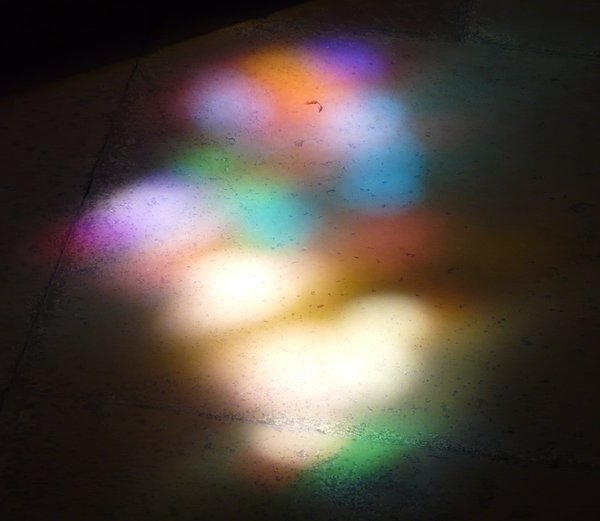
\includegraphics[width=\linewidth]{lichtspiel.jpg}};\end{tcbcliptitle}}]
\lipsum[1]
\end{tcolorbox}
\end{dispExample}
\end{docEnvironment}

\clearpage
\begin{docTcbKey}{clip title}{\colOpt{=true\textbar false}}{默认 |true|，初始 |false|}
  设置将标题裁剪到标题区域范围内。
\begin{dispExample}
\tcbset{enhanced,width=5cm,colframe=red!50!white,coltitle=black,
  colbacktitle=yellow!50!white}

\begin{tcolorbox}[title=\mbox{This is a title which is unbreakable and far too long}]
This is a tcolorbox.
\end{tcolorbox}

\begin{tcolorbox}[title=\mbox{This is a title which is unbreakable and far too long},
  clip title]
This is a tcolorbox.
\end{tcolorbox}
\end{dispExample}
\end{docTcbKey}


\begin{docTcbKey}{clip upper}{\colOpt{=true\textbar false}}{默认 |true|，初始 |false|}
  设置将上部裁剪到内部区域范围内。
\begin{dispExample}
\newcommand{\mygraphics}[2][]{%
  \tcbox[enhanced,boxsep=0pt,top=0pt,bottom=0pt,left=0pt,
    right=0pt,boxrule=0.4pt,drop fuzzy shadow,clip upper,
    colback=black!75!white,toptitle=2pt,bottomtitle=2pt,nobeforeafter,
    center title,fonttitle=\small\sffamily,title=\detokenize{#2}]
  {\includegraphics[width=\the\dimexpr(\linewidth-4mm)/2\relax]{#2}}}

\mygraphics{lichtspiel.jpg}\hfill
\mygraphics{Basilica_5.png}
\end{dispExample}
\end{docTcbKey}

\clearpage
\refKey{/tcb/clip upper} 的示例按图片尺寸确定文本框大小。
若要反过来做（按文本框尺寸确定图片），水印选项提供了一种简便方法。
\begin{dispExample}
\newcommand{\mygraphics}[2][]{%
  \tcbox[enhanced,capture=minipage,boxsep=0pt,top=0pt,bottom=0pt,left=0pt,
    right=0pt,boxrule=0.4pt,drop fuzzy shadow,nobeforeafter,
    colback=black!75!white,toptitle=2pt,bottomtitle=2pt,
    center title,fonttitle=\small\sffamily,title=\detokenize{#2},
    width=(\linewidth-4mm)/2,height=6cm,colbacktitle={black},
    watermark zoom=1.0,watermark graphics={#2}]{}}

\mygraphics{lichtspiel.jpg}\hfill
\mygraphics{Basilica_5.png}
\end{dispExample}


\begin{docTcbKey}{clip lower}{\colOpt{=true\textbar false}}{默认 |true|，初始 |false|}
  设置将下部裁剪到内部区域范围内。
\begin{dispExample}
\tcbset{enhanced,width=5cm,colframe=red!50!black,text and listing}

\begin{tcblisting}{}
Donau\-dampf\-schiff\-fahrts\-ka\-pi\-t\"ans\-m\"ut\-zen\-fran\-sen
\end{tcblisting}

\begin{tcblisting}{clip lower}
Donau\-dampf\-schiff\-fahrts\-ka\-pi\-t\"ans\-m\"ut\-zen\-fran\-sen
\end{tcblisting}
\end{dispExample}
\end{docTcbKey}


\clearpage
\subsection{边线选项键}\label{subsec:borderline}
皮肤 \refSkin{standard} 不支持这些边线，
但其他大多数皮肤（例如 \refSkin{enhanced}）都支持。

边线独立于 |tcolorbox| 的常规框线。
无论是否使用 \refKey{/tcb/segmentation engine}，都可使用它们。

边线可以叠加，即同一个 |tcolorbox| 上可以使用多条不同的边线。
它们在文本框边框和内部绘制\emph{之后}、
覆盖层或水印绘制\emph{之前}绘制。

\begin{marker}
从技术上讲，|tcolorbox| 的常规框线来自 \tikzname\ 的\emph{填充}过程，
而边线则由 \tikzname\ 的\emph{绘制}过程产生。
借此可以实现不同的效果。
\end{marker}


\begin{docTcbKey}{borderline}{=\marg{width}\marg{offset}\marg{options}}{无默认值，初始未设置}
  向边线栈中添加一条新边线。
  该边线以所给 \meta{宽度} 绘制，并相对于边框轮廓计算出一个
  \meta{偏移}。正的 \meta{偏移} 值将边线移向 |tcolorbox| 内部，
  负的 \meta{偏移} 值将其移向外部，且不改变包围盒。\\
  该边线沿一条 \tikzname\ 路径并用所给 \tikzname\ \meta{选项} 绘制。
  注意：此处不应使用 \tikzname\ 的 |line width| 选项。\\
  边线会适应 |tcolorbox| 的圆角。内侧边线必要时会转为尖角，
  外侧边线除使用 \refKey{/tcb/sharp corners} 外始终保持圆角。
\begin{dispExample}
\begin{tcolorbox}[enhanced,title=Rounded corners,fonttitle=\bfseries,boxsep=5pt,
  arc=8pt,
  borderline={0.5pt}{0pt}{red},
  borderline={0.5pt}{5pt}{blue,dotted},
  borderline={0.5pt}{-5pt}{green} ]
This is a tcolorbox.
\end{tcolorbox}
\bigskip
\begin{tcolorbox}[enhanced,title=Sharp corners,fonttitle=\bfseries,boxsep=5pt,
  arc=8pt,sharp corners=downhill,
  borderline={0.5pt}{0pt}{red},
  borderline={0.5pt}{5pt}{blue,dotted},
  borderline={0.5pt}{-5pt}{green} ]
This is a tcolorbox.
\end{tcolorbox}
\end{dispExample}

\begin{dispExample}
% \usepackage{lipsum}
\begin{tcolorbox}[enhanced,arc=3mm,boxrule=1.5mm,boxsep=1.5mm,
  colback=yellow!20!white,
  colframe=blue,
  borderline={1mm}{1mm}{white},
  borderline={1mm}{2mm}{red} ]
  \lipsum[1]
\end{tcolorbox}
\end{dispExample}


\begin{dispExample}
% \usepackage{lipsum}
\begin{tcolorbox}[enhanced,arc=3mm,boxrule=1.5mm,
  frame hidden,colback=blue!10!white,
  borderline={1mm}{0mm}{blue,dotted} ]
  \lipsum[2]
\end{tcolorbox}
\end{dispExample}


\begin{dispExample}
% \usepackage{lipsum}
\begin{tcolorbox}[enhanced,skin=enhancedmiddle,
  frame hidden,interior hidden,top=0mm,bottom=0mm,boxsep=0mm,
  borderline={0.75mm}{0mm}{red},
  borderline={0.75mm}{0.75mm}{red!50!yellow},
  borderline={0.75mm}{1.5mm}{yellow}, ]
  \lipsum[3]
\end{tcolorbox}
\end{dispExample}

\begin{dispExample}
% \usepackage{lipsum}
\newtcolorbox{mygreenbox}[2][]{%
  enhanced,width=\linewidth-6pt,
  enlarge top by=3pt,enlarge bottom by=3pt,
  enlarge left by=3pt,enlarge right by=3pt,
  title={#2},frame hidden,boxrule=0pt,top=1mm,bottom=1mm,
  colframe=green!30!black, colbacktitle=green!50!yellow,
  coltitle=black, colback=green!25!white,
  borderline={0.5pt}{-0.5pt}{green!75!blue},
  borderline={1pt}{-3pt}{green!50!blue},#1}

\begin{mygreenbox}{My title}
  \lipsum[4]
\end{mygreenbox}
\end{dispExample}
\end{docTcbKey}


\begin{docTcbKey}{no borderline}{}{无默认值，初始已设置}
  若此前设置了边线，则将其全部移除。
\end{docTcbKey}


\begin{docTcbKey}{show bounding box}{\colOpt{=\meta{color}}}{默认 |red|，初始未设置}
  显示 |tcolorbox| 的包围盒边线。
  其用途是调试和微调，不应出现在最终文档中。
  可选的 \meta{颜色} 是包围盒边线的基色。
\begin{dispExample}
\tcbset{enhanced,nobeforeafter,width=4cm,fonttitle=\bfseries}

\begin{tcolorbox}[show bounding box,title=Normal]
This is a tcolorbox.
\end{tcolorbox}%
\begin{tcolorbox}[show bounding box=blue,title=Shadow,drop fuzzy shadow]
This is a tcolorbox.
\end{tcolorbox}%
\begin{tcolorbox}[show bounding box=green,title=Enlarged,drop fuzzy shadow,
  enlarge by=2mm]
This is a tcolorbox.
\end{tcolorbox}
\end{dispExample}
\end{docTcbKey}

\clearpage

\begin{marker}
以下\emph{局部}边线的行为与前述完整边线略有不同。
它们忽略圆角设置，其长度不受 \meta{偏移} 影响，
它们忽略皮肤设置，但能适应可断开的文本框。
\end{marker}

\begin{docTcbKey}[][doc new=2014-10-20]{borderline north}{=\marg{width}\marg{offset}\marg{options}}{无默认值，初始未设置}
  在 |tcolorbox| 的北侧添加一条所给 \meta{宽度} 的新边线。
  正的 \meta{偏移} 值将边线移向 |tcolorbox| 内部，
  负的 \meta{偏移} 值将其移向外部，且不改变包围盒。
\begin{dispExample*}{sbs,lefthand ratio=0.6}
\begin{tcolorbox}[enhanced,
  borderline north={2pt}{-2pt}{red}]
  This is a \textbf{tcolorbox}.
\end{tcolorbox}
\end{dispExample*}
\end{docTcbKey}

\begin{docTcbKey}[][doc new=2014-10-20]{borderline south}{=\marg{width}\marg{offset}\marg{options}}{无默认值，初始未设置}
  在 |tcolorbox| 的南侧添加一条所给 \meta{宽度} 的新边线。
  正的 \meta{偏移} 值将边线移向 |tcolorbox| 内部，
  负的 \meta{偏移} 值将其移向外部，且不改变包围盒。
\begin{dispExample*}{sbs,lefthand ratio=0.6}
\begin{tcolorbox}[enhanced,
  borderline south={2pt}{-2pt}{red}]
  This is a \textbf{tcolorbox}.
\end{tcolorbox}
\end{dispExample*}
\end{docTcbKey}

\begin{docTcbKey}[][doc new=2014-10-20]{borderline east}{=\marg{width}\marg{offset}\marg{options}}{无默认值，初始未设置}
  在 |tcolorbox| 的东侧添加一条所给 \meta{宽度} 的新边线。
  正的 \meta{偏移} 值将边线移向 |tcolorbox| 内部，
  负的 \meta{偏移} 值将其移向外部，且不改变包围盒。
\begin{dispExample*}{sbs,lefthand ratio=0.6}
\begin{tcolorbox}[enhanced,
  borderline east={2pt}{-2pt}{red}]
  This is a \textbf{tcolorbox}.
\end{tcolorbox}
\end{dispExample*}
\end{docTcbKey}

\begin{docTcbKey}[][doc new=2014-10-20]{borderline west}{=\marg{width}\marg{offset}\marg{options}}{无默认值，初始未设置}
  在 |tcolorbox| 的西侧添加一条所给 \meta{宽度} 的新边线。
  正的 \meta{偏移} 值将边线移向 |tcolorbox| 内部，
  负的 \meta{偏移} 值将其移向外部，且不改变包围盒。
\begin{dispExample*}{sbs,lefthand ratio=0.6}
\begin{tcolorbox}[enhanced,
  borderline west={2pt}{-2pt}{red}]
  This is a \textbf{tcolorbox}.
\end{tcolorbox}
\end{dispExample*}
\end{docTcbKey}

\clearpage
\begin{docTcbKey}[][doc new=2014-10-20]{borderline horizontal}{=\marg{width}\marg{offset}\marg{options}}{无默认值，初始未设置}
  在 |tcolorbox| 的北侧和南侧各添加一条所给 \meta{宽度} 的新边线。
  正的 \meta{偏移} 值将边线移向 |tcolorbox| 内部，
  负的 \meta{偏移} 值将其移向外部，且不改变包围盒。
\begin{dispExample*}{sbs,lefthand ratio=0.6}
\begin{tcolorbox}[blanker,top=3mm,bottom=3mm,
   borderline horizontal={2pt}{0pt}{red}]
  This is a \textbf{tcolorbox}.
\end{tcolorbox}
\end{dispExample*}
\end{docTcbKey}


\begin{docTcbKey}[][doc new=2014-10-20]{borderline vertical}{=\marg{width}\marg{offset}\marg{options}}{无默认值，初始未设置}
  在 |tcolorbox| 的东侧和西侧各添加一条所给 \meta{宽度} 的新边线。
  正的 \meta{偏移} 值将边线移向 |tcolorbox| 内部，
  负的 \meta{偏移} 值将其移向外部，且不改变包围盒。
\begin{dispExample*}{sbs,lefthand ratio=0.6}
\begin{tcolorbox}[blanker,left=3mm,right=3mm,
   borderline vertical={2pt}{0pt}{red}]
  This is a \textbf{tcolorbox}.\\
  My second line.
\end{tcolorbox}
\end{dispExample*}
\end{docTcbKey}

\begin{dispExample}
\begin{tcolorbox}[enhanced,colback=yellow!10!white,boxrule=0pt,frame hidden,
  borderline north={1mm}{-2mm}{red},
  borderline south={1mm}{-2mm}{blue},
  borderline west={1mm}{-2mm}{green},
  borderline east={1mm}{-2mm}{yellow}]
\lipsum[1]
\end{tcolorbox}
\end{dispExample}

\clearpage
\subsection{阴影选项键}\label{subsec:shadows}
皮肤 \refSkin{standard} 不支持这些阴影，
但其他大多数皮肤（例如 \refSkin{enhanced}）都支持。

阴影可以叠加，即同一个 |tcolorbox| 上可以使用多个不同的阴影。
它们在文本框边框绘制\emph{之前}绘制。

\begin{docTcbKey}{no shadow}{}{无默认值}
  若此前设置了阴影，则将其全部移除。
\end{docTcbKey}

\subsubsection{常见阴影与光晕}

\begin{docTcbKey}{drop shadow}{\colOpt{=\meta{color}}}{样式，默认 |black!50!white|}
  向阴影栈中添加一个标准尺寸的新阴影。
  可按需更改阴影的 \meta{颜色}。
\begin{dispExample*}{sbs,lefthand ratio=0.6}
\tcbset{enhanced,colback=red!5!white,
  colframe=red!75!black,fonttitle=\bfseries}

\begin{tcolorbox}[drop shadow]
This is a tcolorbox.
\end{tcolorbox}\par\bigskip
\begin{tcolorbox}[title=Another shadow,
  drop shadow=blue]
This is a tcolorbox.
\end{tcolorbox}
\end{dispExample*}
\end{docTcbKey}


\begin{docTcbKey}{drop fuzzy shadow}{\colOpt{=\meta{color}}}{样式，默认 |black!50!white|}
  向阴影栈中添加一个标准尺寸的新模糊阴影。
  可按需更改阴影的 \meta{颜色}。
\begin{dispExample*}{sbs,lefthand ratio=0.6}
\tcbset{enhanced,colback=red!5!white,
  colframe=red!75!black,fonttitle=\bfseries}

\begin{tcolorbox}[drop fuzzy shadow]
This is a tcolorbox.
\end{tcolorbox}\par\bigskip
\begin{tcolorbox}[title=Another shadow,
  drop fuzzy shadow=blue]
This is a tcolorbox.
\end{tcolorbox}
\end{dispExample*}
\end{docTcbKey}


\begin{docTcbKey}{drop midday shadow}{\colOpt{=\meta{color}}}{样式，默认 |black!50!white|}
  向阴影栈中添加一个标准尺寸的新阴影。
  可按需更改阴影的 \meta{颜色}。
\begin{dispExample*}{sbs,lefthand ratio=0.6}
\tcbset{enhanced,colback=red!5!white,
  colframe=red!75!black,fonttitle=\bfseries}

\begin{tcolorbox}[drop midday shadow]
This is a tcolorbox.
\end{tcolorbox}\par\bigskip
\begin{tcolorbox}[title=Another shadow,
  drop midday shadow=blue]
This is a tcolorbox.
\end{tcolorbox}
\end{dispExample*}
\end{docTcbKey}

%\enlargethispage*{2cm}
\begin{docTcbKey}{drop fuzzy midday shadow}{\colOpt{=\meta{color}}}{样式，默认 |black!50!white|}
  向阴影栈中添加一个标准尺寸的新模糊阴影。
  可按需更改阴影的 \meta{颜色}。
\begin{dispExample*}{sbs,lefthand ratio=0.6}
\tcbset{enhanced,colback=red!5!white,
  colframe=red!75!black,fonttitle=\bfseries}

\begin{tcolorbox}[drop fuzzy midday shadow]
This is a tcolorbox.
\end{tcolorbox}\par\bigskip
\begin{tcolorbox}[title=Another shadow,
  drop fuzzy midday shadow=blue]
This is a tcolorbox.
\end{tcolorbox}
\end{dispExample*}
\end{docTcbKey}


\begin{docTcbKey}{halo}{\colOpt{=\meta{size} \texttt{with} \meta{color}}}{样式，默认 |0.9mm with yellow|}
  用所给 \meta{颜色} 添加一个新的光晕阴影，
  它在各侧以 \meta{尺寸} 与文本框重叠。
\begin{dispExample*}{sbs,lefthand ratio=0.6}
\tcbset{enhanced,colback=red!5!white,
  colframe=red!75!black,fonttitle=\bfseries}

\begin{tcolorbox}[title=My own halo,halo]
This is a tcolorbox.
\end{tcolorbox}
\par\bigskip\bigskip
\begin{tcolorbox}[title=Another halo,
  halo=2mm with green]
This is a tcolorbox.
\end{tcolorbox}
\end{dispExample*}
\end{docTcbKey}

\enlargethispage*{2cm}
\begin{docTcbKey}{fuzzy halo}{\colOpt{=\meta{size} \texttt{with} \meta{color}}}{样式，默认 |0.9mm with yellow|}
  用所给 \meta{颜色} 添加一个新的模糊光晕阴影，
  它在各侧以 \meta{尺寸} 再加 |0.48mm| 与文本框重叠。
\begin{dispExample*}{sbs,lefthand ratio=0.6}
\tcbset{enhanced,colback=red!5!white,
  colframe=red!75!black,fonttitle=\bfseries}

\begin{tcolorbox}[title=My own halo,fuzzy halo]
This is a tcolorbox.
\end{tcolorbox}
\par\bigskip\bigskip
\begin{tcolorbox}[title=Another halo,
  fuzzy halo=2mm with green]
This is a tcolorbox.
\end{tcolorbox}
\end{dispExample*}

\begin{dispExample}
\begin{tcolorbox}[blank,enhanced jigsaw,boxsep=2pt,arc=2pt,
  fuzzy halo=2mm with red!50!white,
  fuzzy halo=1mm with white]
\lipsum[1]
\end{tcolorbox}
\end{dispExample}
\end{docTcbKey}


\clearpage
对于以下所有阴影，均可像前述示例那样按需更改阴影的 \meta{颜色}。

\begin{docTcbKey}{drop shadow southeast}{\colOpt{=\meta{color}}}{样式，默认 |black!50!white|}
  向阴影栈中添加一个标准尺寸的新阴影。
  本阴影与 \refKey{/tcb/drop shadow} 相同。
\begin{dispExample*}{sbs,lefthand ratio=0.7}
\begin{tcolorbox}[drop shadow southeast,
  enhanced,colback=red!5!white,colframe=red!75!black]
  This is a tcolorbox.
\end{tcolorbox}
\end{dispExample*}
\end{docTcbKey}%

\begin{docTcbKey}{drop shadow south}{\colOpt{=\meta{color}}}{样式，默认 |black!50!white|}
  向阴影栈中添加一个标准尺寸的新阴影。
  本阴影与 \refKey{/tcb/drop midday shadow} 相同。
\begin{dispExample*}{sbs,lefthand ratio=0.7}
\begin{tcolorbox}[drop shadow south,
  enhanced,colback=red!5!white,colframe=red!75!black]
  This is a tcolorbox.
\end{tcolorbox}
\end{dispExample*}
\end{docTcbKey}%

\begin{docTcbKey}{drop shadow southwest}{\colOpt{=\meta{color}}}{样式，默认 |black!50!white|}
  向阴影栈中添加一个标准尺寸的新阴影。
\begin{dispExample*}{sbs,lefthand ratio=0.7}
\begin{tcolorbox}[drop shadow southwest,
  enhanced,colback=red!5!white,colframe=red!75!black]
  This is a tcolorbox.
\end{tcolorbox}
\end{dispExample*}
\end{docTcbKey}%

\begin{docTcbKey}{drop shadow west}{\colOpt{=\meta{color}}}{样式，默认 |black!50!white|}
  向阴影栈中添加一个标准尺寸的新阴影。
\begin{dispExample*}{sbs,lefthand ratio=0.7}
\begin{tcolorbox}[drop shadow west,
  enhanced,colback=red!5!white,colframe=red!75!black]
  This is a tcolorbox.
\end{tcolorbox}
\end{dispExample*}
\end{docTcbKey}%

\begin{docTcbKey}{drop shadow northwest}{\colOpt{=\meta{color}}}{样式，默认 |black!50!white|}
  向阴影栈中添加一个标准尺寸的新阴影。
\begin{dispExample*}{sbs,lefthand ratio=0.7}
\begin{tcolorbox}[drop shadow northwest,
  enhanced,colback=red!5!white,colframe=red!75!black]
  This is a tcolorbox.
\end{tcolorbox}
\end{dispExample*}
\end{docTcbKey}%

\begin{docTcbKey}{drop shadow north}{\colOpt{=\meta{color}}}{样式，默认 |black!50!white|}
  向阴影栈中添加一个标准尺寸的新阴影。
\begin{dispExample*}{sbs,lefthand ratio=0.7}
\begin{tcolorbox}[drop shadow north,
  enhanced,colback=red!5!white,colframe=red!75!black]
  This is a tcolorbox.
\end{tcolorbox}
\end{dispExample*}
\end{docTcbKey}%

\clearpage
\begin{docTcbKey}{drop shadow northeast}{\colOpt{=\meta{color}}}{样式，默认 |black!50!white|}
  向阴影栈中添加一个标准尺寸的新阴影。
\begin{dispExample*}{sbs,lefthand ratio=0.7}
\begin{tcolorbox}[drop shadow northeast,
  enhanced,colback=red!5!white,colframe=red!75!black]
  This is a tcolorbox.
\end{tcolorbox}
\end{dispExample*}
\end{docTcbKey}%

\begin{docTcbKey}{drop shadow east}{\colOpt{=\meta{color}}}{样式，默认 |black!50!white|}
  向阴影栈中添加一个标准尺寸的新阴影。
\begin{dispExample*}{sbs,lefthand ratio=0.7}
\begin{tcolorbox}[drop shadow east,
  enhanced,colback=red!5!white,colframe=red!75!black]
  This is a tcolorbox.
\end{tcolorbox}
\end{dispExample*}
\end{docTcbKey}%


\begin{docTcbKey}{drop fuzzy shadow southeast}{\colOpt{=\meta{color}}}{样式，默认 |black!50!white|}
  向阴影栈中添加一个标准尺寸的新模糊阴影。
  本阴影与 \refKey{/tcb/drop fuzzy shadow} 相同。
\begin{dispExample*}{sbs,lefthand ratio=0.7}
\begin{tcolorbox}[drop fuzzy shadow southeast,
  enhanced,colback=red!5!white,colframe=red!75!black]
  This is a tcolorbox.
\end{tcolorbox}
\end{dispExample*}
\end{docTcbKey}%

\begin{docTcbKey}{drop fuzzy shadow south}{\colOpt{=\meta{color}}}{样式，默认 |black!50!white|}
  向阴影栈中添加一个标准尺寸的新模糊阴影。
  本阴影与 \refKey{/tcb/drop fuzzy midday shadow} 相同。
\begin{dispExample*}{sbs,lefthand ratio=0.7}
\begin{tcolorbox}[drop fuzzy shadow south,
  enhanced,colback=red!5!white,colframe=red!75!black]
  This is a tcolorbox.
\end{tcolorbox}
\end{dispExample*}
\end{docTcbKey}%

\begin{docTcbKey}{drop fuzzy shadow southwest}{\colOpt{=\meta{color}}}{样式，默认 |black!50!white|}
  向阴影栈中添加一个标准尺寸的新模糊阴影。
\begin{dispExample*}{sbs,lefthand ratio=0.7}
\begin{tcolorbox}[drop fuzzy shadow southwest,
  enhanced,colback=red!5!white,colframe=red!75!black]
  This is a tcolorbox.
\end{tcolorbox}
\end{dispExample*}
\end{docTcbKey}%

\begin{docTcbKey}{drop fuzzy shadow west}{\colOpt{=\meta{color}}}{样式，默认 |black!50!white|}
  向阴影栈中添加一个标准尺寸的新模糊阴影。
\begin{dispExample*}{sbs,lefthand ratio=0.7}
\begin{tcolorbox}[drop fuzzy shadow west,
  enhanced,colback=red!5!white,colframe=red!75!black]
  This is a tcolorbox.
\end{tcolorbox}
\end{dispExample*}
\end{docTcbKey}%

\clearpage
\begin{docTcbKey}{drop fuzzy shadow northwest}{\colOpt{=\meta{color}}}{样式，默认 |black!50!white|}
  向阴影栈中添加一个标准尺寸的新模糊阴影。
\begin{dispExample*}{sbs,lefthand ratio=0.7}
\begin{tcolorbox}[drop fuzzy shadow northwest,
  enhanced,colback=red!5!white,colframe=red!75!black]
  This is a tcolorbox.
\end{tcolorbox}
\end{dispExample*}
\end{docTcbKey}%

\begin{docTcbKey}{drop fuzzy shadow north}{\colOpt{=\meta{color}}}{样式，默认 |black!50!white|}
  向阴影栈中添加一个标准尺寸的新模糊阴影。
\begin{dispExample*}{sbs,lefthand ratio=0.7}
\begin{tcolorbox}[drop fuzzy shadow north,
  enhanced,colback=red!5!white,colframe=red!75!black]
  This is a tcolorbox.
\end{tcolorbox}
\end{dispExample*}
\end{docTcbKey}%

\begin{docTcbKey}{drop fuzzy shadow northeast}{\colOpt{=\meta{color}}}{样式，默认 |black!50!white|}
  向阴影栈中添加一个标准尺寸的新模糊阴影。
\begin{dispExample*}{sbs,lefthand ratio=0.7}
\begin{tcolorbox}[drop fuzzy shadow northeast,
  enhanced,colback=red!5!white,colframe=red!75!black]
  This is a tcolorbox.
\end{tcolorbox}
\end{dispExample*}
\end{docTcbKey}%

\begin{docTcbKey}{drop fuzzy shadow east}{\colOpt{=\meta{color}}}{样式，默认 |black!50!white|}
  向阴影栈中添加一个标准尺寸的新模糊阴影。
\begin{dispExample*}{sbs,lefthand ratio=0.7}
\begin{tcolorbox}[drop fuzzy shadow east,
  enhanced,colback=red!5!white,colframe=red!75!black]
  This is a tcolorbox.
\end{tcolorbox}
\end{dispExample*}
\end{docTcbKey}%


\clearpage
\subsubsection{悬浮阴影}

\begin{docTcbKey}{drop lifted shadow}{\colOpt{=\meta{color}}}{样式，默认 |black!50!white|}
  向阴影栈中添加一个标准尺寸的新悬浮阴影。
  可按需更改阴影的 \meta{颜色}。
\begin{dispExample*}{sbs,lefthand ratio=0.6}
\tcbset{enhanced,colback=red!5!white,
  boxrule=0.4pt,sharp corners,
  colframe=red!75!black,fonttitle=\bfseries}

\begin{tcolorbox}[drop lifted shadow]
This is a tcolorbox.
\end{tcolorbox}\par\bigskip
\begin{tcolorbox}[title=Another shadow,
  drop lifted shadow=blue]
This is a tcolorbox.
\end{tcolorbox}
\end{dispExample*}
\end{docTcbKey}


\begin{docTcbKey}{drop small lifted shadow}{\colOpt{=\meta{color}}}{样式，默认 |black!50!white|}
  向阴影栈中添加一个标准尺寸的新小型悬浮阴影。
  可按需更改阴影的 \meta{颜色}。
\begin{dispExample*}{sbs,lefthand ratio=0.6}
\tcbset{enhanced,colback=red!5!white,
  boxrule=0.4pt,sharp corners,
  colframe=red!75!black,fonttitle=\bfseries}

\tcbox[drop small lifted shadow,size=fbox]
  {This is a tcolorbox.}
\par\bigskip
\begin{tcolorbox}[title=Another shadow,
  drop small lifted shadow=black]
This is a tcolorbox.
\end{tcolorbox}
\end{dispExample*}
\end{docTcbKey}


\begin{docTcbKey}{drop large lifted shadow}{\colOpt{=\meta{color}}}{样式，默认 |black!50!white|}
  向阴影栈中添加一个标准尺寸的新大型悬浮阴影。
  可按需更改阴影的 \meta{颜色}。
\begin{dispExample*}{sbs,lefthand ratio=0.6}
\tcbset{enhanced,colback=red!5!white,
  colframe=red!75!black,fonttitle=\bfseries}

\begin{tcolorbox}[drop large lifted shadow]
This is a tcolorbox.
\end{tcolorbox}\par\bigskip
\begin{tcolorbox}[title=Another shadow,
  drop large lifted shadow=blue]
This is a tcolorbox.
\end{tcolorbox}
\end{dispExample*}
\end{docTcbKey}


\clearpage

\subsubsection{通用阴影}
\begin{docTcbKey}{shadow}{=\marg{xshift}\marg{yshift}\marg{offset}\marg{options}}{无默认值}
  向阴影栈中添加一个新阴影。
  该阴影沿 |tcolorbox| 的轮廓绘制，但沿 \meta{xshift} 和 \meta{yshift} 平移。
  \meta{偏移} 值是距边框轮廓的距离。正的 \meta{偏移} 值使阴影缩小，
  负的 \meta{偏移} 值使阴影放大。
  阴影沿一条 \tikzname\ 路径并用所给 \tikzname\ \meta{选项} 填充。\\
  阴影会适应 |tcolorbox| 的圆角。缩小的阴影必要时会转为尖角，
  放大的阴影可能视若干因素变得更圆。但使用 \refKey{/tcb/sharp corners}
  时阴影为尖角。
  \begin{marker}
  默认情况下，包围盒计算不考虑阴影。
  大阴影可能被后续内容覆盖。但必要时可调整包围盒。
  \end{marker}

\begin{dispExample*}{sbs,lefthand ratio=0.6}
\tcbset{enhanced,colback=red!5!white,
  colframe=red!75!black,fonttitle=\bfseries}

\begin{tcolorbox}[title=My own shadow,
  shadow={2mm}{-1mm}{0mm}{black!50!white}]
This is a tcolorbox.
\end{tcolorbox}
\par\bigskip
\begin{tcolorbox}[title=Another shadow,
  shadow={-1mm}{-2mm}{0mm}{fill=blue,
    opacity=0.5}]
This is a tcolorbox.
\end{tcolorbox}
\par\bigskip
\begin{tcolorbox}[title=Double shadow,
  shadow={-1.5mm}{-1.5mm}{0mm}{fill=blue,
    opacity=0.25},
  shadow={1.5mm}{-1.5mm}{0mm}{fill=red,
    opacity=0.25}]
This is a tcolorbox.
\end{tcolorbox}
\par\bigskip
\begin{tcolorbox}[title=Far shadow,
  shadow={5.5mm}{-3.5mm}{2mm}{fill=black,
    opacity=0.25}]
This is a tcolorbox.
\end{tcolorbox}
\par\bigskip\bigskip
\begin{tcolorbox}[title=Halo shadow,
  shadow={0mm}{0mm}{-1.5mm}%
     {fill=yellow!75!red,opacity=0.5}]
This is a tcolorbox.
\end{tcolorbox}
\end{dispExample*}
\end{docTcbKey}

\clearpage
\begin{docTcbKey}{fuzzy shadow}{=\marg{xshift}\marg{yshift}\marg{offset}\marg{step}\marg{options}}{无默认值}
  向阴影栈中添加一个新模糊阴影。实际上，本选项
  会添加若干个阴影，使其看起来像一个边缘模糊的阴影。
  该模糊阴影沿 |tcolorbox| 的轮廓绘制，但沿 \meta{xshift} 和 \meta{yshift} 平移。
  \meta{偏移} 值是距边框轮廓的距离。正的 \meta{偏移} 值使阴影缩小，
  负的 \meta{偏移} 值使阴影放大。
  \marg{步长} 值描述各局部阴影组合时所用的收缩偏移量。
  阴影沿一条 \tikzname\ 路径并用所给 \tikzname\ \meta{选项} 填充，
  但任何 |opacity| 值都会被忽略。
\begin{dispExample*}{sbs,lefthand ratio=0.6}
\tcbset{enhanced,colback=red!5!white,
  colframe=red!75!black,fonttitle=\bfseries}

\begin{tcolorbox}[title=My own shadow,
  fuzzy shadow={2mm}{-1mm}{0mm}{0.1mm}%
               {black!50!white}]
This is a tcolorbox.
\end{tcolorbox}
\par\bigskip
\begin{tcolorbox}[title=Another shadow,
  fuzzy shadow={-1mm}{-2mm}{0mm}{0.2mm}%
               {fill=blue}]
This is a tcolorbox.
\end{tcolorbox}
\par\bigskip
\begin{tcolorbox}[title=Double shadow,
  fuzzy shadow={-1.5mm}{-1.5mm}{0mm}{0.1mm}%
               {blue},
  fuzzy shadow={1.5mm}{-1.5mm}{0mm}{0.1mm}%
               {red}]
This is a tcolorbox.
\end{tcolorbox}
\par\bigskip
\begin{tcolorbox}[title=Far shadow,
  fuzzy shadow={5.5mm}{-3.5mm}{0mm}{0.3mm}%
               {black}]
This is a tcolorbox.
\end{tcolorbox}
\par\bigskip\bigskip
\begin{tcolorbox}[title=Glow shadow,
  fuzzy shadow={0mm}{0mm}{-1.5mm}{0.15mm}%
               {yellow!75!red}]
This is a tcolorbox.
\end{tcolorbox}
\end{dispExample*}

\begin{dispExample}
\newtcolorbox{mybox}[1][]{enhanced,
  fuzzy shadow={1.0mm}{-1.0mm}{0.12mm}{0mm}{blue!50!white},
  fuzzy shadow={-1.0mm}{-1.0mm}{0.12mm}{0mm}{red!50!white},
  fuzzy shadow={-1.0mm}{1.0mm}{0.12mm}{0mm}{green!50!white},
  fuzzy shadow={1.0mm}{1.0mm}{0.12mm}{0mm}{yellow!50!white},#1
}

\begin{mybox}[title=A multi shadow box]
This is a tcolorbox.
\end{mybox}
\end{dispExample}
\end{docTcbKey}


\clearpage
\begin{docTcbKey}[][doc new=2015-05-05]{smart shadow arc}{\colOpt{=true\textbar false}}{默认 |true|，
  初始 |true|}
若设为 |true|，阴影绘制算法会尝试对阴影的弧度做一种较为
聪明的计算。对于常见的圆角文本框效果不错，但对圆形文本框会给出奇怪的结果。

\begin{dispExample}
\tcbset{enhanced,nobeforeafter,colback=red!5!white,
  colframe=red!75!black,width=3cm,square,halign=center,valign=center
  }

\begin{tcolorbox}[drop shadow]
Smart shadow arc (arguably better than normal)
\end{tcolorbox}
\hfill
\begin{tcolorbox}[smart shadow arc=false, drop shadow]
Normal shadow arc
\end{tcolorbox}
\hfill
\begin{tcolorbox}[circular arc, drop shadow]
Smart shadow arc (worse than normal)
\end{tcolorbox}
\hfill
\begin{tcolorbox}[circular arc, smart shadow arc=false, drop shadow]
Normal shadow arc
\end{tcolorbox}
\end{dispExample}
\end{docTcbKey}


\begin{docTcbKey}{lifted shadow}{=\marg{xshift}\marg{yshift}\marg{bend}\marg{step}\marg{options}}{无默认值}
  向阴影栈中添加一个新悬浮阴影。实际上，本选项
  会添加若干个阴影，使其看起来像一个边缘模糊的阴影。
  该悬浮阴影沿 |tcolorbox| 的轮廓绘制，但在左下角沿
  \meta{xshift} 和 \meta{yshift} 平移，在右下角沿
  $-$\meta{xshift} 和 \meta{yshift} 平移。
  此外，中间还有一个 \meta{弯曲量}。
  \marg{步长} 值描述各局部阴影组合时所用的收缩偏移量。
  阴影沿一条 \tikzname\ 路径并用所给 \tikzname\ \meta{选项} 填充，
  但任何 |opacity| 值都会被忽略。
\begin{dispExample*}{sbs,lefthand ratio=0.6}
\tcbset{enhanced,colback=red!5!white,
  boxrule=0.1pt,
  colframe=red!75!black,fonttitle=\bfseries}

\begin{tcolorbox}[title=My own shadow,
  lifted shadow={1mm}{-2mm}{3mm}{0.1mm}%
               {black!50!white}]
This is a tcolorbox.
\end{tcolorbox}
\end{dispExample*}
\end{docTcbKey}

\clearpage
\subsubsection{\tikzname\ 阴影}
除前述宏包自带的阴影选项外，还可使用 \tikzname\ 的
\flqq 阴影程序库\frqq 所提供的阴影。
此类阴影可通过 \refKey{/tcb/frame style} 直接添加到边框路径上。

\begin{exdispExample*}{tikz_shadow_1}{sbs,lefthand ratio=0.7}
% \usetikzlibrary{shadows}
\begin{tcolorbox}[enhanced,
  colback=red!5!white,colframe=red!75!black,
  frame style={drop shadow} ]
  This is a tcolorbox.
\end{tcolorbox}
\end{exdispExample*}

\begin{exdispExample*}{tikz_shadow_2}{sbs,lefthand ratio=0.7}
% \usetikzlibrary{shadows}
\begin{tcolorbox}[enhanced,height=3cm,
  colback=red!5!white,colframe=red!75!black,
  halign=center,valign=center,
  frame style={circular drop shadow} ]
  This is a tcolorbox.
\end{tcolorbox}
\end{exdispExample*}

\begin{exdispExample*}{tikz_shadow_3}{sbs,lefthand ratio=0.7}
% \usetikzlibrary{shadows}
\begin{tcolorbox}[enhanced,width=2.5cm,
  square,circular arc,
  halign=center,valign=center,
  colback=red!5!white,colframe=red!75!black,
  frame style={circular glow={fill=red}} ]
  tcolorbox
\end{tcolorbox}
\end{exdispExample*}


\clearpage
\subsection{\tikzname\ 图片选项键}\label{subsec:tikzpicture}

\begin{docTcbKey}{tikz}{=\meta{tikz option list}}{无默认值，初始为空}
  将所给 \meta{tikz 选项列表} 添加到用于绘制文本框的主 |tikzpicture| 环境中，
  见 \cite{tantau:tikz_and_pgf}。若第二次使用本选项，
  新的 \meta{tikz 选项列表} 会追加到当前选项列表之后。
  注意：若使用 \tikzname\ 坐标变换选项，
  可能还需要 |transform shape| 才能变换所有框元素。
\begin{dispExample*}{sbs,lefthand ratio=0.66,
  segmentation style={preaction={fill=white},pattern=checkerboard,pattern color=gray!40}}
\tcbset{enhanced,colback=red!5!white,
  colframe=red!75!black,fonttitle=\bfseries}

\begin{tcolorbox}[title=Transparent box,
  tikz={opacity=0.5,transparency group}]
This is a tcolorbox.
\end{tcolorbox}
\end{dispExample*}

\begin{dispExample*}{sbs,lefthand ratio=0.66}
\tcbset{enhanced,colback=red!5!white,
  colframe=red!75!black,fonttitle=\bfseries,
  fontupper=\bfseries\Huge,
  halign title=center,halign=center}

\begin{tcolorbox}[title=Rotated box,
  tikz={rotate=30}]
Sold!
\end{tcolorbox}
\end{dispExample*}

\end{docTcbKey}


\begin{docTcbKey}{tikz reset}{}{初始已设置}
  移除 \refKey{/tcb/tikz} 给出的所有选项。
\end{docTcbKey}


\begin{docTcbKey}{at begin tikz}{=\meta{tikz code}}{无默认值，初始为空}
  所给 \meta{tikz 代码} 在 |tikzpicture| 环境开头执行，
  时机为 \tikzname\ 选项 |execute at begin picture| 应用之后。
  若第二次使用本选项，新的 \meta{tikz 代码} 会追加到当前代码之后。
\end{docTcbKey}


\begin{docTcbKey}{at begin tikz reset}{}{初始已设置}
  移除 \refKey{/tcb/at begin tikz} 给出的所有代码。
\end{docTcbKey}


\begin{docTcbKey}{at end tikz}{=\meta{tikz code}}{无默认值，初始为空}
  所给 \meta{tikz 代码} 在 |tikzpicture| 环境末尾执行，
  时机为 \tikzname\ 选项 |execute at end picture| 应用之前。
  若第二次使用本选项，新的 \meta{tikz 代码} 会追加到当前代码之后。
\end{docTcbKey}


\begin{docTcbKey}{at end tikz reset}{}{初始已设置}
  移除 \refKey{/tcb/at end tikz} 给出的所有代码。
\end{docTcbKey}


\clearpage
\begin{docTcbKey}{rotate}{=\meta{angle}}{无默认值，初始未设置}
  将 |tcolorbox| 旋转所给 \meta{角度}。
  同时也会应用 |transform shape|。
  注意：这是一种 \tikzname\ 坐标变换，也就是说，并非所有图形元素（如着色）
  都会真正被旋转。
\begin{dispExample*}{sbs,lefthand ratio=0.66}
\tcbset{enhanced,colback=red!5!white,
  colframe=red!75!black,fonttitle=\bfseries}

\begin{tcolorbox}[title=Rotated box,rotate=30]
This is a tcolorbox.
\end{tcolorbox}
\end{dispExample*}
\end{docTcbKey}

\begin{docTcbKey}{scale}{=\meta{fraction}}{无默认值，初始未设置}
  将 |tcolorbox| 按所给 \meta{比例} 缩放。
  同时也会应用 |transform shape|。
  注意：这是一种 \tikzname\ 坐标变换，也就是说，并非所有图形元素（如线宽）
  都会真正被缩放。
\begin{dispExample*}{sbs,lefthand ratio=0.66}
\tcbset{enhanced,colback=red!5!white,
  colframe=red!75!black,fonttitle=\bfseries}

\begin{tcolorbox}[title=Scaled box,scale=0.5]
This is a tcolorbox.
\end{tcolorbox}
\begin{tcolorbox}[title=Scaled box,scale=1.25]
This is a tcolorbox.
\end{tcolorbox}
\end{dispExample*}
\end{docTcbKey}


\begin{docTcbKey}{remember}{}{样式，初始未设置}
  是 |tikz={remember picture}| 的快捷方式。
  借此可在其他 \tikzname\ 图片中引用节点。
\begin{dispExample}
\begin{tcolorbox}[enhanced,remember,colback=red!5!white,colframe=red!75!black,
  fonttitle=\bfseries,title=The four corners of a paper,
  overlay={\draw[red!50!white,line width=1mm,opacity=0.5,shorten >=3mm]
    (frame.north west) edge[->] (current page.north west)
    (frame.north east) edge[->] (current page.north east)
    (frame.south west) edge[->] (current page.south west)
    (frame.south east) edge[->] (current page.south east);}]
This is a tcolorbox.
\end{tcolorbox}
\end{dispExample}
\end{docTcbKey}

\clearpage
\tcbinterruptdraftmode%
\begin{docTcbKey}{remember as}{=\meta{name}}{样式，无默认值，初始未设置}
  |frame| 节点将以所给 \meta{名称} 记录，以便在其他 \tikzname\ 图片中引用。
\begin{dispExample}
% \usepackage{lipsum}
\newtcolorbox{mybox}[1][]{enhanced,colframe=blue!75!black,colback=blue!10!white,
  fonttitle=\bfseries,#1}

\begin{mybox}[title=First Box,nobeforeafter,width=\linewidth/4,remember as=one]
This is a test.
\end{mybox}
\hfill
\begin{mybox}[title=Second Box,nobeforeafter,width=\linewidth/4,remember as=two]
This is a test.
\end{mybox}
\hfill
\begin{mybox}[title=Third Box,nobeforeafter,width=\linewidth/4,remember as=three]
This is a test.
\end{mybox}

\lipsum[2]

\begin{mybox}[title=Fourth Box,remember as=four]
This is a test.
\end{mybox}

\begin{tikzpicture}[overlay,remember picture,line width=1mm,draw=red!75!black]
  \draw[->] (one.east) to[bend right] node[above] {A} (two.west);
  \draw[->] (two.east) to[bend left] node[above] {B} (three.west);
  \draw[->] (three.east) to[bend left=90] node[right] {C} (four.east);
  \draw[->] (four.west) to[bend left=90] node[left] {D} (one.west);
\end{tikzpicture}
\end{dispExample}
\end{docTcbKey}
\tcbcontinuedraftmode%


\clearpage
\subsection{底层装饰选项键}\label{subsec:skinunderlay}

底层装饰与 \zvref{subsec:overlays} 中介绍的覆盖层十分相似。
底层装饰在边框和内部绘制\emph{之后}、
覆盖层和文字内容绘制\emph{之前}绘制；总体绘制顺序见
\zvref{subsec:tcolorboxdrawing}。

底层装饰与覆盖层的区别如下：
\begin{itemize}
\item 底层装饰不适用于 \refSkin{standard} 和
  \refSkin{standard jigsaw} 皮肤，
  而覆盖层对这些皮肤同样适用。
  \refSkin{spartan} 皮肤支持底层装饰但不支持覆盖层。
  \begin{marker}
  若在 \refSkin{standard} 皮肤下使用底层装饰，它会被静默忽略。
  \end{marker}
\item 底层装饰可以叠加，即同一个 |tcolorbox| 上可以使用多个不同的底层装饰。
  覆盖层默认不可叠加（但可借助 \mylib{hooks} 程序库实现）。
\item 带框标题用底层装饰实现（\zvref{subsec:skinboxedtitle}），
  水印用覆盖层实现（\zvref{subsec:watermarks}）。
\end{itemize}


\begin{docTcbKey}{underlay}{=\meta{graphical code}}{无默认值，初始未设置}
  将 \meta{图形代码} 添加到文本框绘制过程中。该 \meta{图形代码}
  在边框和内部绘制\emph{之后}、文字内容绘制\emph{之前}绘制。
\begin{dispExample}
\newtcolorbox{mybox}[1][]{enhanced,colback=red!5!white,
  colbacktitle=red!85!black!50!white,
  colframe=red!75!black,fonttitle=\bfseries,watermark color=yellow!50!white,
  underlay={\begin{tcbclipinterior}
    \draw[red!40!white,line width=1cm] (interior.south west)--(interior.north east);
    \end{tcbclipinterior}},
  attach boxed title to top center={yshift=-2mm},#1}

\begin{mybox}[title=My box,watermark text=My Watermark]
\lipsum[2]
\end{mybox}
\end{dispExample}
\end{docTcbKey}


\begin{docTcbKey}{no underlay}{}{样式，无默认值，初始已设置}
  若此前设置了底层装饰，则将其移除。
\end{docTcbKey}

\clearpage
\begin{docTcbKey}{underlay broken}{=\meta{graphical code}}{无默认值，初始未设置}
  若文本框设为 \refKey{/tcb/breakable} 且\emph{确实}发生了断开，
  则将 \meta{图形代码} 添加到文本框绘制过程中。
  \refKey{/tcb/underlay} 会覆盖本键。
\end{docTcbKey}

\enlargethispage*{1cm}

\begin{docTcbKey}{underlay unbroken}{=\meta{graphical code}}{无默认值，初始未设置}
  若文本框设为 \refKey{/tcb/breakable} 但实际\emph{并未}断开，
  或文本框设为 \refKey{/tcb/unbreakable}，
  则将 \meta{图形代码} 添加到文本框绘制过程中。
  \refKey{/tcb/underlay} 会覆盖本键。
\end{docTcbKey}

\begin{docTcbKey}{no underlay unbroken}{}{样式，无默认值，初始已设置}
  若此前设置了未断开底层装饰，则将其移除。
\end{docTcbKey}

\begin{docTcbKey}{underlay first}{=\meta{graphical code}}{无默认值，初始未设置}
  若文本框设为 \refKey{/tcb/breakable} 且\emph{确实}发生了断开，
  则将 \meta{图形代码} 添加到断开序列\emph{首段}的文本框绘制过程中。
  \refKey{/tcb/underlay} 会覆盖本键。
\end{docTcbKey}

\begin{docTcbKey}{no underlay first}{}{样式，无默认值，初始已设置}
  若此前设置了首段底层装饰，则将其移除。
\end{docTcbKey}

\begin{docTcbKey}{underlay middle}{=\meta{graphical code}}{无默认值，初始未设置}
  若文本框设为 \refKey{/tcb/breakable} 且\emph{确实}发生了断开，
  则将 \meta{图形代码} 添加到断开序列\emph{中间段}（若有）的文本框绘制过程中。
  \refKey{/tcb/underlay} 会覆盖本键。
\end{docTcbKey}

\begin{docTcbKey}{no underlay middle}{}{样式，无默认值，初始已设置}
  若此前设置了中间段底层装饰，则将其移除。
\end{docTcbKey}

\begin{docTcbKey}{underlay last}{=\meta{graphical code}}{无默认值，初始未设置}
  若文本框设为 \refKey{/tcb/breakable} 且\emph{确实}发生了断开，
  则将 \meta{图形代码} 添加到断开序列\emph{末段}的文本框绘制过程中。
  \refKey{/tcb/underlay} 会覆盖本键。
\end{docTcbKey}

\begin{docTcbKey}{no underlay last}{}{样式，无默认值，初始已设置}
  若此前设置了末段底层装饰，则将其移除。
\end{docTcbKey}

\begin{docTcbKey}{underlay boxed title}{=\meta{graphical code}}{无默认值，初始未设置}
  若文本框带有\emph{带框标题}（见 \zvref{subsec:skinboxedtitle}），
  则将 \meta{图形代码} 添加到带框标题绘制\emph{之前}的
  文本框绘制过程中。
\end{docTcbKey}

\begin{docTcbKey}{no underlay boxed title}{}{样式，无默认值，初始已设置}
  若此前设置了带框标题底层装饰，则将其移除。
\end{docTcbKey}

\begin{docTcbKey}{underlay unbroken and first}{=\meta{graphical code}}{无默认值，初始未设置}
  这是同时设置
  \refKey{/tcb/underlay unbroken} 和
  \refKey{/tcb/underlay first} 的简写。
  \refKey{/tcb/underlay} 会覆盖本键。
\end{docTcbKey}

\begin{docTcbKey}{underlay middle and last}{=\meta{graphical code}}{无默认值，初始未设置}
  这是同时设置
  \refKey{/tcb/underlay middle} 和
  \refKey{/tcb/underlay last} 的简写。
  \refKey{/tcb/underlay} 会覆盖本键。
\end{docTcbKey}

\begin{docTcbKey}{underlay unbroken and last}{=\meta{graphical code}}{无默认值，初始未设置}
  这是同时设置
  \refKey{/tcb/underlay unbroken} 和
  \refKey{/tcb/underlay last} 的简写。
  \refKey{/tcb/underlay} 会覆盖本键。
\end{docTcbKey}

\begin{docTcbKey}[][doc new=2014-09-19]{underlay first and middle}{=\meta{graphical code}}{无默认值，初始未设置}
  这是同时设置
  \refKey{/tcb/underlay first} 和
  \refKey{/tcb/underlay middle} 的简写。
  \refKey{/tcb/underlay} 会覆盖本键。
\end{docTcbKey}


\clearpage
\subsection{收尾装饰选项键}\label{subsec:skinfinish}

收尾装饰与 \zvref{subsec:skinunderlay} 介绍的底层装饰
以及 \zvref{subsec:overlays} 介绍的覆盖层十分相似。
收尾装饰在文字内容绘制\emph{之后}绘制；总体绘制顺序见
\zvref{subsec:tcolorboxdrawing}。因此，收尾装饰会降低文字内容的可读性。

收尾装饰用于特殊效果，例如高亮、光泽或文字叠文字。

\begin{itemize}
\item 收尾装饰仅适用于以下皮肤：
  \refSkin{enhanced}、
  \refSkin{empty}、
  \refSkin{freelance}、
  \refSkin{bicolor}、
  \refSkin{beamer} 和
  \refSkin{widget}。
  \begin{marker}
  若在 \refSkin{standard} 皮肤下使用收尾装饰，它会被静默忽略。
  \end{marker}
\item 收尾装饰可以叠加，即同一个 |tcolorbox| 上可以使用多个不同的收尾装饰。
\end{itemize}

\enlargethispage*{2cm}
\begin{docTcbKey}{finish}{=\meta{graphical code}}{无默认值，初始未设置}
  将 \meta{图形代码} 添加到文本框绘制过程中。该 \meta{图形代码}
  在文字内容绘制\emph{之后}绘制。
\begin{dispExample}
\newtcolorbox{mybox}[1][]{enhanced,colback=red!5!white,
  colbacktitle=red!85!black!50!white,colframe=red!75!black,fonttitle=\bfseries,
  finish={\begin{tcbclipframe}
    \path[bottom color=black,top color=black!50!white,opacity=0.1]
      (frame.south west) -- (frame.south east) -- (frame.north east) -- cycle;
    \path[top color=white,bottom color=black!50!white,opacity=0.1]
      (frame.south west) -- (frame.north east) -- (frame.north west) -- cycle;
    \end{tcbclipframe}},#1}

\begin{mybox}[title=My box]
\lipsum[2]
\end{mybox}
\end{dispExample}
\begin{dispExample}
\newtcolorbox{mybox}[1][]{enhanced,colback=red!5!white,
  colbacktitle=red!85!black!50!white,colframe=red!75!black,fonttitle=\bfseries,
  finish={\node[draw,fill=white,fill opacity=0.85,inner sep=5mm,
    rounded corners] at (frame.center) {\Huge\bfseries Finish!};},#1}

\begin{mybox}[title=My box]
\lipsum[2]
\end{mybox}
\end{dispExample}
\end{docTcbKey}

\clearpage
\begin{docTcbKey}{no finish}{}{样式，无默认值，初始已设置}
  若此前设置了收尾装饰，则将其移除。
\end{docTcbKey}


\begin{docTcbKey}{finish broken}{=\meta{graphical code}}{无默认值，初始未设置}
  若文本框设为 \refKey{/tcb/breakable} 且\emph{确实}发生了断开，
  则将 \meta{图形代码} 添加到文本框绘制过程中。
  \refKey{/tcb/finish} 会覆盖本键。
\end{docTcbKey}

\begin{docTcbKey}{finish unbroken}{=\meta{graphical code}}{无默认值，初始未设置}
  若文本框设为 \refKey{/tcb/breakable} 但实际\emph{并未}断开，
  或文本框设为 \refKey{/tcb/unbreakable}，
  则将 \meta{图形代码} 添加到文本框绘制过程中。
  \refKey{/tcb/finish} 会覆盖本键。
\end{docTcbKey}

\begin{docTcbKey}{no finish unbroken}{}{样式，无默认值，初始已设置}
  若此前设置了未断开收尾装饰，则将其移除。
\end{docTcbKey}

\begin{docTcbKey}{finish first}{=\meta{graphical code}}{无默认值，初始未设置}
  若文本框设为 \refKey{/tcb/breakable} 且\emph{确实}发生了断开，
  则将 \meta{图形代码} 添加到断开序列\emph{首段}的文本框绘制过程中。
  \refKey{/tcb/finish} 会覆盖本键。
\end{docTcbKey}

\begin{docTcbKey}{no finish first}{}{样式，无默认值，初始已设置}
  若此前设置了首段收尾装饰，则将其移除。
\end{docTcbKey}

\begin{docTcbKey}{finish middle}{=\meta{graphical code}}{无默认值，初始未设置}
  若文本框设为 \refKey{/tcb/breakable} 且\emph{确实}发生了断开，
  则将 \meta{图形代码} 添加到断开序列\emph{中间段}（若有）的文本框绘制过程中。
  \refKey{/tcb/finish} 会覆盖本键。
\end{docTcbKey}

\begin{docTcbKey}{no finish middle}{}{样式，无默认值，初始已设置}
  若此前设置了中间段收尾装饰，则将其移除。
\end{docTcbKey}

\begin{docTcbKey}{finish last}{=\meta{graphical code}}{无默认值，初始未设置}
  若文本框设为 \refKey{/tcb/breakable} 且\emph{确实}发生了断开，
  则将 \meta{图形代码} 添加到断开序列\emph{末段}的文本框绘制过程中。
  \refKey{/tcb/finish} 会覆盖本键。
\end{docTcbKey}

\begin{docTcbKey}{no finish last}{}{样式，无默认值，初始已设置}
  若此前设置了末段收尾装饰，则将其移除。
\end{docTcbKey}

\begin{docTcbKey}{finish unbroken and first}{=\meta{graphical code}}{无默认值，初始未设置}
  这是同时设置
  \refKey{/tcb/finish unbroken} 和
  \refKey{/tcb/finish first} 的简写。
  \refKey{/tcb/finish} 会覆盖本键。
\end{docTcbKey}

\begin{docTcbKey}{finish middle and last}{=\meta{graphical code}}{无默认值，初始未设置}
  这是同时设置
  \refKey{/tcb/finish middle} 和
  \refKey{/tcb/finish last} 的简写。
  \refKey{/tcb/finish} 会覆盖本键。
\end{docTcbKey}

\begin{docTcbKey}{finish unbroken and last}{=\meta{graphical code}}{无默认值，初始未设置}
  这是同时设置
  \refKey{/tcb/finish unbroken} 和
  \refKey{/tcb/finish last} 的简写。
  \refKey{/tcb/finish} 会覆盖本键。
\end{docTcbKey}


\begin{docTcbKey}[][doc new=2014-09-19]{finish first and middle}{=\meta{graphical code}}{无默认值，初始未设置}
  这是同时设置
  \refKey{/tcb/finish first} 和
  \refKey{/tcb/finish middle} 的简写。
  \refKey{/tcb/finish} 会覆盖本键。
\end{docTcbKey}

\clearpage
\subsection{超链接选项键}\label{subsec:hyper}
本节所有选项都需要单独加载 \refPkg{hyperref} 宏包 \cite{rahtz:hyperref}。
这些选项均以 \refKey{/tcb/finish} 形式实现，
可用 \refKey{/tcb/no finish} 禁用。

\begin{marker}
若未加载 \refPkg{hyperref} 宏包 \cite{rahtz:hyperref}，或使用了
\refSkin{standard} 皮肤，则所有超链接选项都会被静默忽略。
\end{marker}

\begin{docTcbKey}[][doc new=2017-02-03]{hyperref}{=\meta{marker}}{无默认值，初始未设置}
  将 |tcolorbox| 的整个\textit{边框}设为指向某个 \meta{标记} 的活动超链接，
  该标记由 |\label|、\refKey{/tcb/label} 或 \refKey{/tcb/phantomlabel} 给出。
  这样，|tcolorbox| 就成了一个可点击按钮（取决于预览器）。
  \begin{dispExample*}{sbs,lefthand ratio=0.7}
% \section{Library skins}\label{sec:skins}%
\begin{tcolorbox}[beamer,colback=red!50,
  hyperref=sec:skins]
Jump to the heading of Section~\ref*{sec:skins}.
\end{tcolorbox}
  \end{dispExample*}
\end{docTcbKey}

\begin{docTcbKey}[][doc new=2017-02-03]{hyperref interior}{=\meta{marker}}{无默认值，初始未设置}
  与 \refKey{/tcb/hyperref} 相同，但仅将 |tcolorbox| 的\textit{内部}
  设为超链接（不含边框和标题）。
\end{docTcbKey}

\begin{docTcbKey}[][doc new=2017-02-03]{hyperref title}{=\meta{marker}}{无默认值，初始未设置}
  与 \refKey{/tcb/hyperref} 相同，但仅将 |tcolorbox| 的\textit{标题}
  设为超链接。
\end{docTcbKey}

\begin{docTcbKey}[][doc new=2017-02-03]{hyperref node}{=\marg{marker}\marg{node}}{无默认值，初始未设置}
  与 \refKey{/tcb/hyperref} 相同，但仅将所给的 \tikzname\ \meta{节点}
  设为超链接。该 \meta{节点} 可以是 |frame|、|interior|、|title|，
  或用于绘制 |tcolorbox| 的任何其他命名节点。
  \meta{节点} 可定义在 \refKey{/tcb/underlay}、\refKey{/tcb/overlay}
  或 \refKey{/tcb/finish} 内部。若使用后者，请在应用
  \refKey{/tcb/hyperref node}\emph{之前}定义该节点。
  \begin{dispExample*}{sbs,lefthand ratio=0.7}
% \section{Library skins}\label{sec:skins}%
\begin{tcolorbox}[enhanced,colback=yellow!10,
  underlay={\node[red,fill=red!30,inner sep=3mm]
   (click) at (frame.center) {X};},
  hyperref node={sec:skins}{click}]
Jump to the heading of Section~\ref*{sec:skins}
(X marks the click point).
\end{tcolorbox}
  \end{dispExample*}
\end{docTcbKey}

\begin{docTcbKey}[][doc new=2017-02-03]{hyperlink}{=\meta{marker}}{无默认值，初始未设置}
  将 |tcolorbox| 的整个\textit{边框}设为指向某个 \meta{标记} 的活动超链接，
  该标记由 |\hypertarget| 或 \refKey{/tcb/hypertarget} 给出。
  这样，|tcolorbox| 就成了一个可点击按钮（取决于预览器）。
  \begin{dispExample*}{sbs,lefthand ratio=0.7}
% \usepackage{hyperref}%
\begin{tcolorbox}[enhanced,
  colback=blue!10,colframe=blue!50!black,
  hypertarget=hypertwinB,
  hyperlink=hypertwinA,
  title=Box B]
Click me to jump to Box A.
\end{tcolorbox}
  \end{dispExample*}
\end{docTcbKey}

\clearpage
\begin{docTcbKey}[][doc new=2017-02-03]{hyperlink interior}{=\meta{marker}}{无默认值，初始未设置}
  与 \refKey{/tcb/hyperlink} 相同，但仅将 |tcolorbox| 的\textit{内部}
  设为超链接（不含边框和标题）。
\end{docTcbKey}

\begin{docTcbKey}[][doc new=2017-02-03]{hyperlink title}{=\meta{marker}}{无默认值，初始未设置}
  与 \refKey{/tcb/hyperlink} 相同，但仅将 |tcolorbox| 的\textit{标题}
  设为超链接。
\end{docTcbKey}

\begin{docTcbKey}[][doc new=2017-02-03]{hyperlink node}{=\marg{marker}\marg{node}}{无默认值，初始未设置}
  与 \refKey{/tcb/hyperlink} 相同，但仅将所给的 \tikzname\ \meta{节点}
  设为超链接。该 \meta{节点} 可以是 |frame|、|interior|、|title|，
  或用于绘制 |tcolorbox| 的任何其他命名节点。
  \meta{节点} 可定义在 \refKey{/tcb/underlay}、\refKey{/tcb/overlay}
  或 \refKey{/tcb/finish} 内部。若使用后者，请在应用
  \refKey{/tcb/hyperlink node}\emph{之前}定义该节点。
\end{docTcbKey}

\begin{docTcbKey}[][doc new=2017-02-03]{hyperurl}{=\meta{url}}{无默认值，初始未设置}
  将 |tcolorbox| 的整个\textit{边框}设为指向某个 \meta{url} 的活动超链接，
  方式与使用 |\href| 或 |\url| 相同。
  这样，|tcolorbox| 就成了一个可点击按钮（取决于预览器）。
  \begin{dispExample*}{sbs,lefthand ratio=0.7}
\begin{tcolorbox}[enhanced,colback=red!50,
  hyperurl=https://www.ctan.org/pkg/tcolorbox]
View CTAN with a browser.
\end{tcolorbox}
  \end{dispExample*}
\end{docTcbKey}

\begin{docTcbKey}[][doc new=2017-02-03]{hyperurl interior}{=\meta{url}}{无默认值，初始未设置}
  与 \refKey{/tcb/hyperurl} 相同，但仅将 |tcolorbox| 的\textit{内部}
  设为超链接（不含边框和标题）。
\end{docTcbKey}

\begin{docTcbKey}[][doc new=2017-02-03]{hyperurl title}{=\meta{url}}{无默认值，初始未设置}
  与 \refKey{/tcb/hyperurl} 相同，但仅将 |tcolorbox| 的\textit{标题}
  设为超链接。
\end{docTcbKey}

\begin{docTcbKey}[][doc new=2017-02-03]{hyperurl node}{=\marg{url}\marg{node}}{无默认值，初始未设置}
  与 \refKey{/tcb/hyperurl} 相同，但仅将所给的 \tikzname\ \meta{节点}
  设为超链接。该 \meta{节点} 可以是 |frame|、|interior|、|title|，
  或用于绘制 |tcolorbox| 的任何其他命名节点。
  \meta{节点} 可定义在 \refKey{/tcb/underlay}、\refKey{/tcb/overlay}
  或 \refKey{/tcb/finish} 内部。若使用后者，请在应用
  \refKey{/tcb/hyperurl node}\emph{之前}定义该节点。
\end{docTcbKey}


\begin{docTcbKey}[][doc new=2017-02-03]{hyperurl*}{=\marg{options}\marg{url}}{无默认值，初始未设置}
  与 \refKey{/tcb/hyperurl} 相同，但额外应用
  \refPkg{hyperref} \cite{rahtz:hyperref} 的 \meta{选项}。
  \begin{dispExample*}{sbs,lefthand ratio=0.7}
\begin{tcolorbox}[enhanced,colback=green!50,
  hyperurl*={page=3,pdfnewwindow=true}%
            {tcolorbox-example.pdf}]
Open example file on Page~3.
\end{tcolorbox}
  \end{dispExample*}
\end{docTcbKey}

\begin{docTcbKey}[][doc new=2017-02-03]{hyperurl* interior}{=\marg{options}\marg{url}}{无默认值，初始未设置}
  与 \refKey{/tcb/hyperurl interior} 相同，但额外应用 |hyperref| \cite{rahtz:hyperref}
  的 \meta{选项}。
\end{docTcbKey}

\begin{docTcbKey}[][doc new=2017-02-03]{hyperurl* title}{=\marg{options}\marg{url}}{无默认值，初始未设置}
  与 \refKey{/tcb/hyperurl title} 相同，但额外应用 |hyperref| \cite{rahtz:hyperref}
  的 \meta{选项}。
\end{docTcbKey}

\enlargethispage*{1cm}

\begin{docTcbKey}[][doc new=2017-02-03]{hyperurl* node}{=\marg{options}\marg{url}\marg{node}}{无默认值，初始未设置}
  与 \refKey{/tcb/hyperurl node} 相同，但额外应用 |hyperref| \cite{rahtz:hyperref}
  的 \meta{选项}。
\end{docTcbKey}



\clearpage
\subsection{拼图皮肤变体}\label{subsec:skinjigsaw}
如 \zvref{sec:skincorekeys} 所述，|tcolorbox| 最多由四个\emph{引擎}绘制。
通常，\emph{边框}引擎用颜色填满整个文本框区域，其他引擎再用别的颜色
填充特定区域。最终，只有你所看到的文本框\emph{边框}区域才显示边框色。
对大多数应用而言，这是一种好方法。

但对某些文本框，需要更精细的处理。例如，若文本框需要半透明，
已经填好色的区域无法再变成未填充。因此，更精巧的边框引擎会在边框上
"挖洞"，让内部区域和可选的标题区域填色透出。
由此得到的皮肤称为\emph{拼图}皮肤。对于 \refSkin{standard}、
\refSkin{enhanced} 和 \refSkin{bicolor}，分别有对应的变体
\refSkin{standard jigsaw}、\refSkin{enhanced jigsaw} 和 \refSkin{bicolor jigsaw}。


\begin{dispExample*}{segmentation style={preaction={fill=white},pattern=checkerboard,pattern color=gray!40}}
\newcommand{\ballexample}{\begin{tikzpicture}
  \path[use as bounding box] (0,0.8) rectangle +(0.1,0.1);
  \shadedraw [shading=ball] (0,0) circle (1cm);
  \shadedraw [ball color=red] (3,-2.2) circle (1cm);
\end{tikzpicture}}

\tcbset{enhanced,colback=blue!5!white,
  frame style={left color=red!75!black,right color=red!10!yellow},
  fonttitle=\bfseries }

\ballexample

\begin{tcolorbox}[title=A normal box]
  \lipsum[2]
\end{tcolorbox}

\ballexample

\begin{tcolorbox}[title=A translucent jigsaw box,
  enhanced jigsaw,opacityback=0.35]
  \lipsum[2]
\end{tcolorbox}
\end{dispExample*}


\begin{dispExample*}{segmentation style={preaction={fill=white},pattern=checkerboard,pattern color=gray!40}}
\tcbset{enhanced,colback=red!10!white,coltitle=black,
  frame style={left color=red!75!black,right color=red!10!yellow},
  fonttitle=\bfseries,interior hidden,title hidden}

\begin{tcolorbox}[title=A normal box with hidden interior and title]
  This is a tcolorbox.
\end{tcolorbox}

\begin{tcolorbox}[enhanced jigsaw,
  title=A jigsaw box with hidden interior and title]
  This is a tcolorbox.
\end{tcolorbox}
\end{dispExample*}


\begin{dispExample*}{segmentation style={preaction={fill=white},pattern=checkerboard,pattern color=gray!40}}
\newtcolorbox{mybox}{skin=enhancedmiddle jigsaw,leftrule=5mm,rightrule=5mm,
  boxsep=0mm,top=0mm,bottom=0mm,
  frame style={top color=blue,bottom color=red},interior hidden}

\begin{mybox}
  \lipsum[2]
\end{mybox}
\end{dispExample*}


\clearpage
\subsection{草稿模式}\label{subsec:draftmode}
在文档起草阶段，可启用\emph{草稿模式}以缩短编译时间。
它基本上会把所有皮肤改为 \refSkin{spartan}，
并将 \refKey{/tcb/fit algorithm} 设为 |squeeze|。
特别是使用模糊阴影时，提速会相当显著。

\begin{marker}
强烈建议最终文档\emph{不要}使用草稿模式。若想一直使用它，请直接使用
\refSkin{spartan}。草稿模式的实现将来可能会变化。
\end{marker}

\begin{marker}
通常情况下，切换到草稿模式不应改变文档的版面几何。
由于覆盖层被停用，放置在其中的任何代码
（例如计数器变更）将不再执行！此外，\refKey{/tcb/remember as}
也不会产生任何效果。你可以使用
\refCom{tcbinterruptdraftmode} / \refCom{tcbcontinuedraftmode}
将关键代码排除在草稿模式转换之外。
\end{marker}


\begin{docCommand}{tcbstartdraftmode}{}
  此后的所有 |tcolorbox| 代码都进入\emph{草稿模式}。
  所有皮肤设置都被 \refSkin{spartan} 覆盖。
  覆盖层、水印、阴影、边线和圆角对所有 |tcolorbox| 层都被停用。
\end{docCommand}

\begin{docCommand}{tcbstopdraftmode}{}
  对之后的代码停用\emph{草稿模式}。
\end{docCommand}

\begin{docCommand}{tcbinterruptdraftmode}{}
  若当前正处于\emph{草稿模式}，则停用\emph{草稿模式}，
  直到遇到随后的 \refCom{tcbcontinuedraftmode}。\par
  若当前不处于\emph{草稿模式}，则什么也不发生，随后的
  \refCom{tcbcontinuedraftmode} 也不会启动\emph{草稿模式}。
  \begin{marker}
  |\tcbinterruptdraftmode| 与 |\tcbcontinuedraftmode| 这一对命令不能嵌套使用。
  \end{marker}
\end{docCommand}

\begin{docCommand}{tcbcontinuedraftmode}{}
  继续由此前的 \refCom{tcbinterruptdraftmode} 暂停的\emph{草稿模式}。
  若 \refCom{tcbinterruptdraftmode} 之前并未处于草稿模式，则什么也不发生。
  \begin{marker}
  位于 \refCom{tcbinterruptdraftmode} 与 \refCom{tcbcontinuedraftmode}
  之间的代码不受\emph{草稿模式}影响。
  \end{marker}
\end{docCommand}


\clearpage

\begin{docTcbKey}{draftmode}{\colOpt{=true\textbar false}}{默认 |true|，初始 |false|}
  若设为 |true|，则启动\emph{草稿模式}。
  若设为 |false|，则停止\emph{草稿模式}。

\begin{dispExample*}{}
\newtcolorbox{mybeamer}[2][]{beamer,colback=Salmon!50!white,
  colframe=FireBrick!75!black,adjusted title={#2},#1}

\begin{mybeamer}{Beamer box}
This box looks like a box provided by the \texttt{beamer} class.
\end{mybeamer}\par\medskip
\begin{mybeamer}[draftmode]{Beamer box}
This box looks like a box provided by the \texttt{beamer} class.
\end{mybeamer}
\end{dispExample*}
\end{docTcbKey}


